% characters_at_aP -- caracteres en las potencias del elemento a_P de Kostant.  8 de septiembre de 2026.
% Carles Marin + Claude (asistente IA).
%
% REGLA DE REDACCION: ni una segunda persona en todo el documento.  Lo unico que se dice de un
% tercero es lo que esta en un articulo publicado suyo, con su localizador.
%
% Compilar:  pdflatex note2 (x2)
\documentclass[11pt,a4paper]{article}
\usepackage[T1]{fontenc}
\usepackage[utf8]{inputenc}
\usepackage{lmodern}
\usepackage[margin=2.6cm]{geometry}
\usepackage{amsmath,amssymb,amsthm}
\usepackage{mathrsfs}
\usepackage{graphicx}
\usepackage{booktabs}
\usepackage[dvipsnames,table]{xcolor}
\usepackage{colortbl}
\usepackage[colorlinks=true,linkcolor=NavyBlue,citecolor=NavyBlue,urlcolor=NavyBlue]{hyperref}
\usepackage{float}
\usepackage{longtable}
% ⚠ colocacion de flotantes: con los valores por defecto una figura a \textwidth con
%   pie largo no cabe con texto debajo y salta de pagina, dejando la anterior corta.
%   Medido: 257 pt de hueco en la p.13 antes de tocar esto.
\renewcommand{\textfraction}{0.07}
\renewcommand{\topfraction}{0.92}
\renewcommand{\bottomfraction}{0.92}
\renewcommand{\floatpagefraction}{0.78}
\usepackage{microtype}

\definecolor{azul}{HTML}{1F4E79}
\definecolor{naranja}{HTML}{C55A11}
\definecolor{filaclara}{HTML}{F2F6FA}
\definecolor{cabecera}{HTML}{DCE6F1}
\definecolor{marca}{HTML}{FBE9DD}

\newtheorem{theorem}{Theorem}[section]
\newtheorem{proposition}[theorem]{Proposition}
\newtheorem{corollary}[theorem]{Corollary}
\newtheorem{observation}[theorem]{Observation}
\newtheorem{lemma}[theorem]{Lemma}
\theoremstyle{definition}
\newtheorem{question}[theorem]{Question}

\newcommand{\Sp}{\mathrm{Sp}}
\newcommand{\SL}{\mathrm{SL}}
\newcommand{\GL}{\mathrm{GL}}
\newcommand{\SO}{\mathrm{SO}}
\newcommand{\cls}{\mathrm{cls}}
\newcommand{\hgt}{\mathrm{ht}}   % \ht es primitiva de TeX: NO redefinir
\newcommand{\rhoh}{\rho^{\vee}}
\newcommand{\ZZ}{\mathbb{Z}}
% el \penalty0 deja que la linea rompa ANTES del marcador
\newcommand{\ver}[1]{\unskip\penalty0\ \textcolor{azul}{\small\textsf{[#1]}}}

% FICHA destacada: fondo tenue + barra vertical de color.  Se mide con lrbox para que la barra
% tenga exactamente la altura del contenido, sin paquetes externos.
\definecolor{fondoficha}{HTML}{EEF3F8}
\newsavebox{\fichabox}
\newenvironment{keybox}
  {\par\vspace{9pt}\begin{lrbox}{\fichabox}%
   \begin{minipage}{0.90\textwidth}\vspace{7pt}\setlength{\parskip}{3pt}}
  {\vspace{7pt}\end{minipage}\end{lrbox}%
   % ⚠ centrado dentro de un \hbox del ancho del texto: con \hfill...\hfill seguido de
   %   \par, el \parfillskip que TeX anade al cerrar el parrafo se suma al \hfill de la
   %   derecha y la ficha se iba a la izquierda.  Se vio mirando la pagina, no el codigo.
   \par\noindent\hbox to \textwidth{\hfill
   \textcolor{azul}{\rule[-\dp\fichabox]{3.2pt}{\dimexpr\ht\fichabox+\dp\fichabox\relax}}%
   \colorbox{fondoficha}{\usebox{\fichabox}}\hfill}%
   \par\vspace{9pt}}

% El subtitulo de 60 palabras se retiro el 10-sep-2026, al preparar el envio a revista: sus cinco
% clausulas --- las cuatro familias, que las potencias de a_P son una de ellas, el valor con su
% signo, la factorizacion en dimensiones y el recuento cerrado --- estan todas en el abstract, de
% modo que no se pierde nada y el titulo deja de leerse como el de un preprint.
\title{\vspace{-1.4cm}\Large Integer character values on the $\rho$-line of $\Sp(2m)$}
\author{\normalsize Carles Mar\'in\thanks{Independent researcher, \texttt{karlesmarin@gmail.com}.
Written with Claude (Anthropic) as a research assistant; every statement was checked by the author.}}
\date{\normalsize 8 September 2026}

\begin{document}
\maketitle
\thispagestyle{empty}

\begin{abstract}
\noindent \textbf{Where this comes from.} In 1940 Littlewood observed that a Schur polynomial
evaluated at a full set of roots of unity either vanishes or factors, and that which of the two
happens is decided by a purely combinatorial datum of the indexing partition. Two traditions grew
out of that observation and have run alongside each other ever since without quite meeting. On one
side, representation theory asks for the value of a character at a distinguished element of the
group: Kostant's 1976 paper singles out two such elements, $a_Q$ and $a_P$, and proves that at
either of them every character is $0$ or $\pm1$. On the other, combinatorics asks the same question
of symmetric functions specialised at roots of unity, and answers it with cores and quotients of
partitions. The first line runs Kostant, Cellini--M\"oseneder Frajria--Papi,
Kumar--Lusztig--Prasad, Prasad, L\"ubeck--Prasad, Nadimpalli--Pattanayak--Prasad; the second runs
Adin--Frumkin, Lecouvey, P\'etr\'eolle, Ayyer--Kumari, Albion, Kumari. Figure~\ref{fig:map} draws
both.

\smallskip
\noindent \textbf{And where it goes.} At $a_P$ itself the question is settled, and settled on
both lines. This note is about the rest of the line. The step away from $a_P$ is not cosmetic:
there the half-sum $\rho$ is a regular point of the relevant arrangement, and the argument that
settles the character is an argument about alcoves that needs exactly that regularity. At the
powers $\rho$ moves onto the walls, the alcove argument degenerates, and the values --- which
were $0$ and $\pm1$ --- run to $72$ one power later in a group of rank three. Further out it is
regular again: no positive root of $C_m$ takes a value above $2\rho_1=2m$, so no $q>2m$ divides
one, and the line has three regimes rather than two. What replaces the
alcove argument, which points of the line still admit an answer at all, and what that answer
looks like, is the content below.

\smallskip
\noindent \textbf{Three things are proved.} The first is a \textbf{classification}: of all the
rational points $g_{1/q}$ of the line, exactly four families have the property that \emph{every}
character of $\Sp(2m)$ takes an integer value there, namely $q\mid 2m$, $q\mid 2m+1$, $q\mid2m+2$,
and a sporadic $q=6$ (Theorem~\ref{thm:clasif}); the argument is that integrality forces the
characteristic polynomial of the natural representation into $\ZZ[X]$, so the spectrum must be
stable under the Galois group; classifying the stable spectra is then elementary. \textbf{The powers of $a_P$ are
the family $q\mid 2m+2$}, and they are no longer the boundary of what can be said but one case of a
list.

\smallskip
\noindent The second is a \textbf{vanishing criterion}: writing $\ell=\lambda+\rho$ and $N_q(x)$ for
the number of positive roots $\alpha$ with $q\mid(x,\alpha)$, the character survives exactly when
$N_q(\ell)=r_q:=N_q(\rho)$. \textbf{At $a_P$ itself that statement is not new, and not new on this
very line}: it is Corollary~3.2 of Cellini--M\"oseneder Frajria--Papi \cite{CMP06}, in every type,
together with the sign; in the coroot statistic it is Corollary~3.7 of
Nadimpalli--Pattanayak--Prasad \cite{NPP25}, for every positive integer. What is left, and what
this note is about, is the \emph{powers}: at $a_P^{\,k}$ with $\gcd(k,2m+2)>1$ the half-sum $\rho$
is no longer regular --- it lies on $r_q$ walls --- and the alcove argument that settles $a_P$
degenerates exactly there. \S\ref{sec:crit} sets the three side by side.

\smallskip
\noindent The third is the value itself, in type $C$, and it is now complete. For every power,
\[
\chi_\lambda(a_P^{\,k})\;=\;(-1)^{E_{p,q}(\lambda)}\,\frac{Z_q(\lambda+\rho)}{Z_q(\rho)}
\]
on the surviving weights and $0$ elsewhere (Theorem~\ref{thm:signo}), with $Z_q$ a product of root
statistics and $E_{p,q}$ a sum of floors --- equivalently a count of three indicators on the residues of $\ell$
taken in order; and that modulus factors as a product of
\textbf{dimensions of irreducible representations of $GL_n$, $Sp_{2n}$ and $SO_{2n+1}$}, one per
folded class (Theorem~\ref{thm:dims}) --- the three types Lecouvey \cite{Lec07a} already reads off
the folded classes of the \emph{full} alphabet, here surviving the deletion of the two letters. Two closed counts of the surviving weights follow
for \emph{every} $q$ (\S\ref{sec:cuenta}), and $G_2$ is done in closed form at $q=3$
(\S\ref{sec:g2}). Nothing above rests on a measurement: the one step that did, the triviality of the
non-vanishing factor, is Proposition~\ref{prop:res}. What is left open is stated in
\S\ref{sec:preguntas}, and it is no longer the value.
\end{abstract}

\begin{center}\small
\emph{2020 Mathematics Subject Classification.}\;
Primary 20G05; Secondary 05E05, 05E10, 05A15, 17B22, 11R18.

\smallskip
\emph{Key words and phrases.}\;
Weyl character formula; classical groups; characters at elements of finite order; Kostant's element
$a_P$; roots of unity; integrality; vanishing criterion; factorisation into dimensions; symplectic
group.
\end{center}

\begin{keybox}
\textbf{In words, before any notation.} A character of a compact group, evaluated at one element of
it, is a single number. This note answers two questions about that number: \emph{when is it zero},
and \emph{what is it when it is not}.

\smallskip
The first answer is a count. Write $\ell=\lambda+\rho$, fix the denominator $q$, count the positive roots
$\alpha$ for which $(\ell,\alpha)$ is divisible by $q$, and compare with the same count on $\rho$.
The count can never come out below; the character is non-zero exactly when it comes out equal.

\smallskip
\textbf{What is new here and what is not.} \emph{At $a_P$ itself, nothing.} The count and the sign
there are Corollary~3.2 of \cite{CMP06}, in every type and on this line; read on \emph{coroots} the
count is Corollary~3.7 of \cite{NPP25}; the principal specialisation the argument runs on is
classical; and at $q=2$ the factorisation into dimensions is Theorem~5.1 of \cite{Kar24}. What is
done here is the \emph{powers}: to identify the alphabet of $a_P^{\,k}$ with the alphabet of
Theorem~2 of \cite{Prasad16b} folded and short of two letters --- which turns out to be the
condition, and not merely a description; to carry the count to the powers, where $\rho$ is no longer
regular; and, in type $C$, to evaluate the character exactly --- sign included --- to factor it into
dimensions at $q\ge3$, and to count the survivors in closed form. The table on
p.~\pageref{tab:attrib} says which is which, line by line.
\end{keybox}

\section{Where this sits}\label{sec:map}

Two literatures have been circling this object for eighty years without quite meeting, and it is
worth one page to say which is which, because the gap is the reason the statements below had not
been made together.

Read the upper line of Figure~\ref{fig:map} from left to right and the object never changes: an
element, and what its centraliser does to a character. Kostant \cite{Kostant76} fixes the two
elements in 1976 and proves that the values are $0$ and $\pm1$. Kumar--Lusztig--Prasad \cite{KLP09}
make \emph{twisted} and \emph{folded} the same word in 2009. Prasad's two papers of 2016 supply
first the geometry of $\rho$ and the Coxeter element \cite{Prasad16}, and then --- this is the
theorem the alphabet of \S\ref{sec:alph} is folded against --- the residue criterion on $\GL_n$
\cite{Prasad16b}. L\"ubeck--Prasad \cite{LP20} carry it to the symmetric and hyperoctahedral groups,
and the line arrives in 2025 at \cite{NPP25} and \cite{Polo25}.

Read the lower line and the object is a partition and its cores. It starts earlier --- Littlewood
\cite{Li40}, 1940 --- and has been running alongside ever since: Adin--Frumkin \cite{AF02} in 2002,
P\'etr\'eolle \cite{Petreolle15} and Wahiche \cite{Wahiche23} on the Macdonald identity of type
$\widetilde C$, Ayyer--Kumari \cite{AK22} and Albion \cite{Alb23} on characters twisted by roots of
unity, Kumari \cite{Kum24} again in 2024. My own two papers \cite{OP1,OP2} are on that side.

\begin{figure}[tbp]
\centering
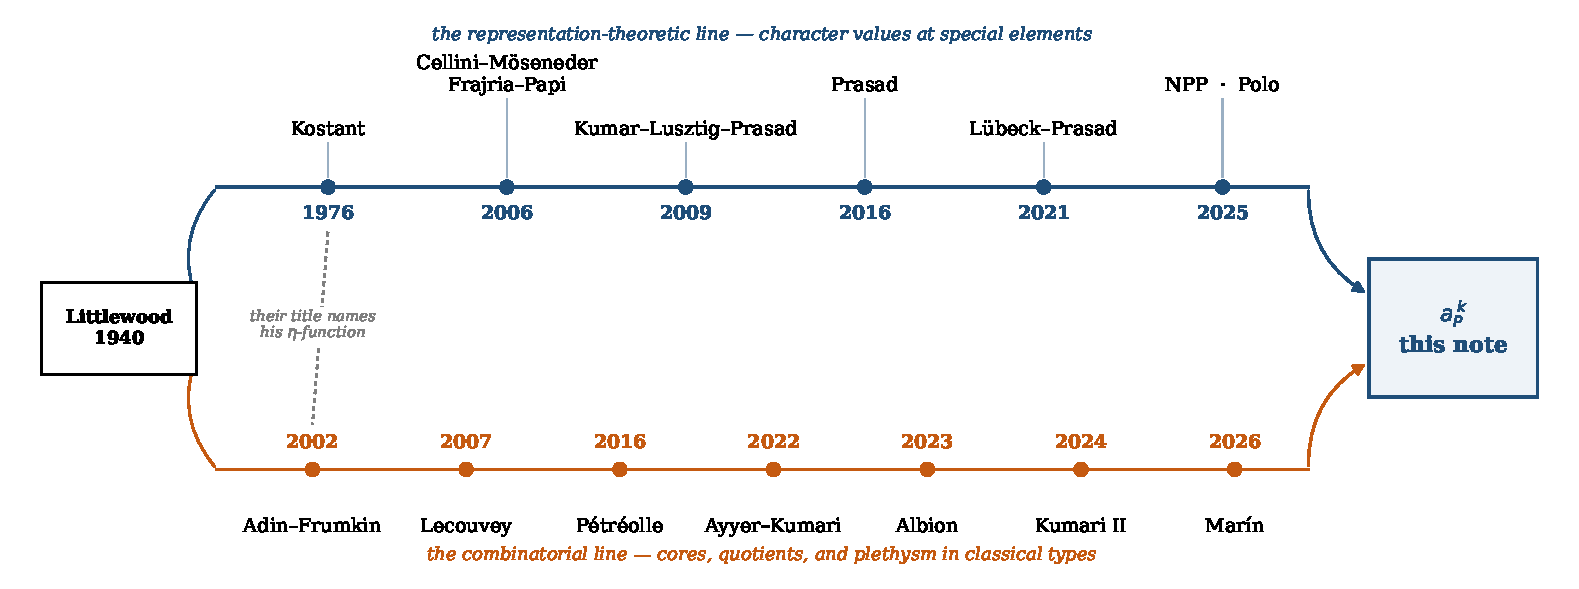
\includegraphics[width=\textwidth]{fig_map.pdf}
\caption{\textbf{The two lines.} The axis is time and each node carries a name and its year of
\emph{publication}, the dates being those of the bibliography below. Above, character values at
special elements: Kostant \cite{Kostant76} fixes $a_Q$ and $a_P$ and proves the values are
$\{0,\pm1\}$; Cellini--M\"oseneder Frajria--Papi \cite{CMP06} evaluate the character at $a_P$
outright; Kumar--Lusztig--Prasad \cite{KLP09} make \emph{twisted} and \emph{folded} the same word;
Prasad \cite{Prasad16,Prasad16b} supplies the geometry of $\rho$ and the residue criterion on
$\GL_n$; L\"ubeck--Prasad \cite{LP20} carry it to $S_{2n}$ and $B_n$; and NPP \cite{NPP25} and Polo
\cite{Polo25} arrive in 2025. Below, the combinatorial side: cores in type $A$
\cite{AF02}; the $\ell$-quotient in classical types through plethysm \cite{Lec07a,Lec07b}; the
Macdonald identity of type $\widetilde C$ \cite{Petreolle15}; and characters twisted by roots of
unity \cite{AK22,Alb23,Kum24}. Littlewood 1940 sits outside both because it feeds both, and the box
on the right is this note: the two arrows into it are the two things it needs, the element from
above and the alphabet from below.
\textbf{The node to read first is 2006.} Corollary~3.2 of \cite{CMP06} is already the vanishing
criterion \emph{and} the sign, in every type, and on the \emph{root} statistic --- this line, not
the coroot line. Everything this note has to add begins one step further along: at the powers
$a_P^{\,k}$, where $\rho$ stops being regular. In the coroot statistic the criterion is
Corollary~3.7 of \cite{NPP25}, for every integer.
The dotted edge is the crossing of 2002: Adin--Frumkin's title is \emph{Rim hook tableaux and
Kostant's $\eta$-function coefficients}, a combinatorial paper taking its coefficients from the 1976
paper where both of Kostant's elements are defined. The two lines do see each other, and it is worth
being exact about how much: \cite{NPP25} cites Ayyer--Kumari; Kumari's papers are motivated by a
conjecture of Wagh and Prasad; and Ayyer--Kumari \cite{AK22} open by saying that Littlewood and
Prasad considered their factorisations \emph{``motivated by a celebrated result of Kostant''}. So the
connection Prasad--Kostant is on the record on both sides. What is \emph{not} on either side is the
identification of \S\ref{sec:alph}: $a_P^{\,k}$ as $d\cdot\mu_q$ less two letters, read on the line
of $\rho$. \ver{figs.py}}
\label{fig:map}
\end{figure}

\section{Normalisations, and which element this is}\label{sec:norm}

The whole note turns on one axis --- roots against coroots --- so the normalisations are fixed
first, and with more care than the object seems to need.

Let $G$ be simple and simply connected with maximal torus $T$, roots $\Phi$, positive roots
$\Phi^+$, and $\rho$ the half-sum of $\Phi^+$. Normalise the invariant form so that short roots have
$(\alpha,\alpha)=2$, and write $\rho^\sharp$ for the vector of $\mathfrak t$ that the form
identifies with $\rho$. For a real parameter $\theta$ put
\begin{equation}\label{eq:gtheta}
g_\theta \;=\; \exp\bigl(2\pi i\,\theta\,\rho^\sharp\bigr)\;\in\;T ,
\end{equation}
so that a weight $\mu$ takes the value $e^{2\pi i\theta(\mu,\rho)}$ on $g_\theta$. Throughout,
$\theta=p/q$ in lowest terms, and \textbf{$q$ is the denominator of the parameter}, which is the
integer every count below is taken modulo.

\begin{keybox}
\textbf{$q$ need not be the order of $g_\theta$, and $\rho^\sharp$ need not be a cocharacter.} In
$A_1$ with $(\alpha,\alpha)=2$ one has $\rho=\omega$ and $(\omega,\rho)=\tfrac12$, so the standard
representation would take the values $z^{\pm1/2}$: the map $z\mapsto\rho(z)$ is a cocharacter of the
adjoint group, not of $SL_2$. Concretely $g_{1/q}=\operatorname{diag}(e^{\pi i/q},e^{-\pi i/q})$ has
order $2q$ in $SL_2$, not $q$. Nothing below is affected --- every statement is about the
\emph{denominator} $q$ --- but the two must not be confused: for
$\operatorname{diag}(i,-i)$, of order $4$, the standard character vanishes, and a count run with
$q=4$ in this normalisation does not see it.
\end{keybox}

\noindent \textbf{In type $C$}, which is where everything after \S\ref{sec:cap} takes place, no such
care is needed. In $\Sp(2m)$ we have $\rho=(m,m-1,\dots,1)$ in the standard coordinates, the
subgroup $\theta\mapsto g_\theta$ has eigenvalues $e^{\pm2\pi i\theta j}$, and with
\[
t=2m+2,\qquad d=\gcd(k,t),\qquad q=t/d,\qquad p=k/d,
\]
Kostant's second element is $a_P=g_{1/t}=\rho(\zeta_t)$, and
\[
a_P^{\,k}=\rho(\zeta_t^{\,k})=\rho(\xi_q),\qquad \xi_q=\zeta_t^{\,k}\ \text{a primitive $q$-th root of
unity},
\]
so that evaluating \eqref{eq:ps} at $\xi_q$ computes $\chi_\lambda(a_P^{\,k})$: that is the whole
bridge, and it is the one place where the parameter and the element are tied together. The relation
$q\mid 2m+2$ belongs to type $C$ and to the powers of $a_P$; it is not part of any general
statement below. \emph{Checked on the $140$ pairs with $2\le m\le11$, $1\le k\le14$: the spectrum
of $g_{p/q}$ is the alphabet of Proposition~\ref{prop:alph} and $\zeta_t^{\,k}$ has order exactly
$q$.} \ver{revision\_52\_bisagra.py}

\section{The criterion, and what of it is already in print}\label{sec:crit}

\subsection*{The identity}

The classical principal specialisation is usually written on the line of $\rho^\vee$, with the
coroot statistic $\langle\lambda+\rho,\alpha^\vee\rangle$. Written on the line of $\rho$ it reads
\begin{equation}\label{eq:ps}
\boxed{\;\chi_\lambda(g_\theta)\;=\;e^{-2\pi i\theta(\lambda,\rho)}\prod_{\alpha>0}
\frac{1-e^{2\pi i\theta(\lambda+\rho,\,\alpha)}}{1-e^{2\pi i\theta(\rho,\,\alpha)}}\;}
\end{equation}
with the \emph{root} statistic. It needs no faith: with $\ell=\lambda+\rho$,
$\sum_w\epsilon(w)z^{(w\ell,\rho)}=\sum_w\epsilon(w)z^{(w\rho,\ell)}$ since
$(w\ell,\rho)=(\ell,w^{-1}\rho)$ and $\epsilon(w)=\epsilon(w^{-1})$; the Weyl denominator identity
turns the right-hand side into $z^{(\rho,\ell)}\prod_{\alpha>0}(1-z^{-(\ell,\alpha)})$; and dividing
by the same computation at $\ell=\rho$ gives \eqref{eq:ps}. All that has changed from the usual form
is which of the two lines one stands on --- which is precisely the axis that separates Kostant's two
elements. \emph{Checked against the bialternant on the $\rho$-line for $m=2,3,4$ to $10^{-12}$.}
\ver{revision\_47\_verificacion.py}

\subsection*{The count}

\begin{theorem}[the criterion]\label{thm:crit}
Let $\lambda$ be dominant, $\ell=\lambda+\rho$, $\theta=p/q$ in lowest terms, and put
\[
N_q(x)=\#\{\alpha>0:\ q\mid(x,\alpha)\},\qquad r_q=N_q(\rho) .
\]
Then $N_q(\ell)\ge r_q$ for every $\lambda$, and
\begin{equation}\label{eq:crit}
\boxed{\;\chi_\lambda(g_{p/q})\neq0 \iff N_q(\ell)=r_q\;}
\end{equation}
\end{theorem}

\begin{proof}
Each factor $1-z^{r}$ of \eqref{eq:ps} has a simple zero at a primitive $q$-th root of unity exactly
when $q\mid r$, so at $z=e^{2\pi ip/q}$ the numerator vanishes to order $N_q(\ell)$ and the
denominator to order $r_q$. A character has no poles, so the first order is at least the second; and
the limit is non-zero exactly when they agree.
\end{proof}

\noindent Nothing in that proof uses $q\mid 2m+2$, or type $C$, or that $p=1$: the statement is about
the whole line $\theta\mapsto g_\theta$, at every rational parameter. The powers of $a_P$ in
$\Sp(2m)$ are the sub-family $q\mid 2m+2$. \emph{Measured on $\mathbf{27\,183}$ dominant weights in
$\Sp(2m)$, $m=2,\dots,6$ and $q=2,\dots,14$, no exception --- and $\mathbf{19\,986}$ of them have
$q\nmid t$. The naive condition ``some root divides'', run as a decoy over the same weights, fails
$7\,968$ times, so the test discriminates; no value was numerically ambiguous.}
\ver{rho\_line\_any\_q.py}

\subsection*{What is already in print, and what is not}

\begin{keybox}
\textbf{The same count, on the other line, is Corollary~3.7 of \cite{NPP25}}, and it must be read
before the above is read as new. In their notation, for every positive integer $m$ and every
dominant $\lambda$:
\[
\#\{\alpha\in\Phi^+ : m\mid\langle\rho,\alpha^\vee\rangle\}\;\le\;
\#\{\alpha\in\Phi^+ : m\mid\langle\lambda+\rho,\alpha^\vee\rangle\},
\]
\emph{and $\Theta_\lambda(\rho^\vee(e^{2\pi i/m}))\neq0$ if and only if that inequality is an
equality.} Their Proposition~3.8 then reads the two sides as dimensions of centralisers in the dual
group, and credits the minimality to Serre.

\smallskip
\textbf{So the difference is the statistic, and therefore the element.} Theorem~\ref{thm:crit} is
the count on $(\,\cdot\,,\alpha)$ --- the line of $\rho$, where $a_P$ lives --- and theirs is the
count on $\langle\,\cdot\,,\alpha^\vee\rangle$ --- the line of $\rho^\vee$, where the Coxeter element
lives. \textbf{In the simply-laced types the two statements coincide} under the normalisation of
\S\ref{sec:norm}, and there Theorem~\ref{thm:crit} is theirs. They part company exactly in the
non-simply-laced types, which is exactly where $a_P$ and $a_Q$ part company, and that is the case
this note is about.
\end{keybox}

\noindent What is left, then, and what the rest of the note is: the identification of the alphabet
(\S\ref{sec:alph}), the translation into capacities in type $C$ (\S\ref{sec:cap}), the exact value
with its sign (\S\ref{sec:valor}), the modulus and its lemma (\S\ref{sec:modulo}), the
factorisation into dimensions (\S\ref{sec:dims}), the counts
(\S\ref{sec:cuenta}) and $G_2$ (\S\ref{sec:g2}).

\section{Why the two tables look alike: the alphabet}\label{sec:alph}

\noindent\emph{Two tables written in two literatures that never cite each other have the same shape. Is that a resemblance, or are they about the same object?}

They look alike because the alphabets are the same object. This is the one place where I can replace
the resemblance by an identity, and it is elementary.

\begin{proposition}\label{prop:alph}
Let $t=2m+2$, $d=\gcd(k,t)$ and $q=t/d$. As a multiset, the symplectic alphabet of $a_P^k$, that is
$A=\{\zeta^{\pm jk}: j=1,\dots,m\}$ with $\zeta$ of order $t$, satisfies
\[
A \;=\; d\cdot\mu_q \;-\; 2\cdot\{1\} \quad (d \text{ even}),
\qquad
A \;=\; d\cdot\mu_q \;-\;\{1\}-\{-1\} \quad (d \text{ odd}).
\]
\end{proposition}

\begin{proof}
Since $t=2m+2$, the exponents $\{\pm j : j=1,\dots,m\}$ are exactly $\ZZ/t\smallsetminus\{0,t/2\}$.
The map $e\mapsto\zeta^{ke}$ factors through $\ZZ/q$, because $\zeta^k$ has order $q$, and every
residue mod $q$ is the image of exactly $d$ elements of $\ZZ/t$; hence
$\{\zeta^{ke}: e\in\ZZ/t\}=d\cdot\mu_q$. It remains to delete the two excluded exponents. For $e=0$
the element is $1$. For $e=t/2=dq/2$: if $d$ is even this is $\equiv 0 \pmod q$ and the element is
again $1$; if $d$ is odd then $q$ is even, since $dq=t$ is, and $dq/2\equiv q/2$, so the element is
$-1$.
\end{proof}

\noindent Before the consequences, an attribution that belongs here. The \emph{undeleted}
alphabet $d\cdot\mu_q$ is not virgin ground on my side of the map either: Ayyer and Kumari
\cite{AK22} treat exactly the symplectic character of $\Sp_{2t'n}$ at $\omega^j x_i$ --- $t'$ being
their order of $\omega$, and $n$ their number of variables --- which at $x_i=1$ is $\mu_{t'}$ with
multiplicity $2n$, counting each eigenvalue with its reciprocal. They give both a vanishing
criterion and a factorisation into characters of smaller classical groups. Their multiplicity is
therefore always even, and nothing is deleted. So the
big alphabet is done on both sides of the map; what is not done is the two points.

Two consequences, and the first is the dictionary.

\begin{keybox}
The alphabet in Theorem~2 of \cite{Prasad16b} at $t=1$ --- the $t$ of that paper, the element of
$\GL_m$, not the $t=2m+2$ of this note --- is $\mu_n$ with multiplicity $m$. The one here is $\mu_q$
with multiplicity $d$, \emph{minus two points}. So the $m$ there is the $d$ here and the $n$ there is
the $q$ here --- not by
analogy but because the multisets are the same one --- and the two missing points
are fixed points of $w\mapsto w^{-1}$ --- one copy of each of the two when $d$ is odd, two copies of
the single one $w=1$ when $d$ is even.
\end{keybox}

\noindent That settles the first three rows of the table on page~1, and it says exactly where the
orange row comes from: the difference between the two criteria is the difference between the two
alphabets, which is two points. Computing the effect of removing them is a deletion problem --- a
symplectic branching literally only when $d$ is even, for the reason set out in the second box
below --- and I did not manage it --- but it turned out not to be needed for the vanishing, which Corollary~\ref{conj:cap}
settles by another route. It is still the natural way in for the \emph{value}, and \S\ref{sec:cierre}
comes back to it.

The second consequence is the generating function, which is what makes everything computable:
\[
H(z)=\frac{(1-z)^2}{(1-z^q)^d}\quad (d\text{ even}),
\qquad
H(z)=\frac{1-z^2}{(1-z^q)^d}\quad (d\text{ odd}),
\]
so the $h_n$ are integers --- supported on the residues $0,1,2$ mod $q$ when $d$ is even and on
$0,2$ when $d$ is odd --- and every determinant in this note is exact. Both statements checked
against the alphabet computed directly, and the version with the parity of $d$ reversed agrees in
$0$ of $72$ cases. \ver{aP\_alfabeto.py}

\noindent What the deletion \emph{is}, geometrically, depends on the parity of $d$, and it took a
wrong version of this paragraph to see why.

\begin{keybox}
\textbf{Unconditionally:} the element of $\GL_t$ of \cite{Prasad16b} has alphabet $d\cdot\mu_q$, and the alphabet of
$a_P^{\,k}$ in $\Sp(t-2)$ is that with exactly two letters deleted --- for $d$ even, two copies of
the fixed point $1$; for $d$ odd, one copy of each of the two fixed points $1$ and $-1$.

\smallskip
\textbf{Only for $d$ even} can that be read as removing a symplectic plane. For $d$ odd it cannot:
then $q$ is even, the eigenvalues $1$ and $-1$ each occur in $d\cdot\mu_q$ with multiplicity $d$,
which is odd, and $\det(d\cdot\mu_q)=(-1)^{d}=-1$, so \emph{no} element of $\Sp(t)$ has that
spectrum; nor is $\{1,-1\}$, of determinant $-1$, a symplectic plane. The smallest case is $d=1$,
$q=6$: the product over $\mu_6$ is $-1$, so $\mu_6$ is not a spectrum in $\Sp(6)$ --- while
$\mu_6\smallsetminus\{1,-1\}$ is one in $\Sp(4)$.
\end{keybox}

\noindent So the two sides are joined by an identity of alphabets, not always by an identity of
elements, and $d$ odd --- which includes $a_P$ itself --- is precisely where the geometric picture
fails. That also removes the easy explanation of the capacities: they cannot simply be blamed on
``the two fixed points'', since for $d$ even only one fixed point is involved, twice.

What that leaves is no longer vague. The deletion of the two letters acts on the
generating function by a single factor, so at the level of the $h_n$ it is a finite difference:
\[
h^{A} = (1-S)^2\,h' \quad (d \text{ even}), \qquad h^{A} = (1-S^2)\,h' \quad (d \text{ odd}),
\]
where $h'_n=\mathbf{1}_{q\mid n}\binom{n/q+d-1}{d-1}$ are those of \cite{Prasad16b} --- the indicator matters, since $h'_n=0$ unless $q\mid n$ --- and $S$ is the shift. So the gap between this note and a
derivation is exactly one question: \emph{what does a second difference of the $h$-sequence do to the
Jacobi--Trudi determinant?} I took it for an obstruction, and it is not one: it comes out as a
product of one-variable operators, in two lines, and \S\ref{sec:cierre} does it. What that still
leaves --- the cancellation among the shifted determinants --- is where this note stops.


\section{Which points of the line have whole answers}\label{sec:clasif}

\noindent\emph{Proposition~\ref{prop:alph} read the alphabet of $a_P^{\,k}$ as a whole multiple of
$\mu_q$ short of two letters. Every point of the line has an alphabet, and for most of them it is
not of that shape. What is special about the ones that are?}

\smallskip
\noindent In general, with $m=uq+v$, the alphabet is $2u\cdot\mu_q$ with a segment
$\{\pm1,\dots,\pm v\}$ added, and Proposition~\ref{prop:alph} is the case where that segment closes
up. The right question is not which alphabets look tidy but which ones the arithmetic cannot tell
apart from their own Galois conjugates --- and that turns out to be a statement about the
characters, not about the notation: whether they are \emph{whole numbers}. The criterion of
\S\ref{sec:crit} holds at every rational point, so nothing so far has forced the family
$q\mid 2m+2$ that the rest of this note evaluates. This is what picks it out.

\begin{theorem}[which denominators give integer values]\label{thm:clasif}
Let $m\ge2$ and $\gcd(p,q)=1$. Then $\chi_\lambda(g_{1/q})\in\ZZ$ for \emph{every} dominant weight
$\lambda$ if and only if at least one of
\[
q\mid 2m,\qquad q\mid 2m+1,\qquad q\mid 2m+2,\qquad q=6 \text{ and } m\equiv1 \!\!\pmod 3
\]
holds; and in that case $g_{p/q}$ is conjugate to $g_{1/q}$ for every $p$ coprime to $q$, so no
character value depends on the numerator.
\end{theorem}

\noindent The word \emph{every} carries the statement. This is not a classification of when one
character happens to come out whole --- that happens all over the line --- but of when all of them
do at once.

\begin{proof}[The argument, which never looks at a weight]
Suppose every $\chi_\lambda(g_{1/q})$ is an integer. The exterior powers
$\Lambda^j\mathbb{C}^{2m}$ are direct sums of irreducibles --- not irreducible themselves ---
so their characters are
$\ZZ$-combinations of the $\chi_\lambda$ and are therefore integers as well; and those
characters are the coefficients of the characteristic polynomial of $g_{1/q}$ acting on
$\mathbb{C}^{2m}$; so that polynomial lies in $\ZZ[X]$,
and the multiplicities of its roots are constant along Galois orbits. Conversely, if the spectrum is
carried to itself by every $\xi_q\mapsto\xi_q^{\,p}$, then $g_{p/q}$ and $g_{1/q}$ have the same
spectrum and are conjugate in $\Sp(2m)$; the character values are then algebraic integers fixed by
the Galois group of $\mathbb{Q}(\xi_q)$, hence rational integers.

What is left is elementary. Write $m=uq+v$ with $0\le v<q$ and $a=\lfloor(q-1)/2\rfloor$. The
spectrum of the natural representation is $\{\xi_q^{\pm j}: j=1,\dots,m\}$, which as a multiset of
$\mu_q$ is
\[
2u\cdot\mu_q \;+\;\{\pm1,\dots,\pm v\} ,
\]
and the first summand is Galois-stable on its own. So the question is when the segment
$\{\pm1,\dots,\pm v\}$ is, and that is a question about residues and nothing else. Sufficiency is
immediate for $v=0$, $v=a$, $v=q-1$ and, when $q$ is even, $v=q/2$: each of those segments is
carried to itself by every $\xi_q\mapsto\xi_q^{\,p}$. Necessity is the step that has to be argued.

Write $A_v=\sum_{j=1}^{v}(\xi_q^{\,j}+\xi_q^{-j})$. If the segment is stable then $A_v$ is fixed by
the whole group; only that direction is used, and it is used in the contrapositive. A full turn sums to zero, whence $A_v+A_{q-1-v}=-2$ and
$\mathbb{Q}(A_v)=\mathbb{Q}(A_w)$ for $w=\min(v,q-1-v)$; the four segments just listed are $w=0$
and $w=a$, so only $1\le w<a$ is left. There set
$\beta_w=1+A_w=\sum_{j=-w}^{w}\xi_q^{\,j}$, a Dirichlet kernel, whose conjugates are
\[
  \sigma_p(\beta_w)=\frac{\sin\bigl((2w+1)\pi p/q\bigr)}{\sin(\pi p/q)} .
\]
For $q\ge4$, $2\le N\le q-2$ and $1\le r\le q-1$ with $r\neq1,q-1$, one has the \emph{strict}
inequality
\[
  \Bigl|\frac{\sin(N\pi r/q)}{\sin(\pi r/q)}\Bigr|
  \;<\;\frac{\sin(N\pi/q)}{\sin(\pi/q)} .
\]
Indeed, replacing $N$ by $n=\min(N,q-N)$ changes no modulus; on $0<x<\pi/n$ the function
$f(x)=\sin(nx)/\sin x$ is positive and strictly decreasing, since $f'/f=n\cot(nx)-\cot x<0$ because
$t\cot t$ decreases on $(0,\pi)$; and on $\pi/n\le x\le\pi/2$ one has
$|f(x)|\le 1/\sin(\pi/n)<1/\sin(\pi/2n)=f(\pi/2n)\le f(\pi/q)$. Taking $N=2w+1$, which lies in that
range precisely when $1\le w<a$, the only automorphisms fixing $\beta_w$ are the identity and
complex conjugation; so $\mathbb{Q}(\beta_w)=\mathbb{Q}(\xi_q+\xi_q^{-1})$, which is $\mathbb{Q}$
only when $\varphi(q)=2$. Inside this range that leaves $q=6$, $w=1$ --- the two segments
$(q,v)=(6,1)$ and $(6,4)$. Translating the surviving residues into divisibilities gives the four
conditions.
\end{proof}

\noindent \emph{Measured on $\mathbf{11\,800}$ pairs $(m,q)$ with $q\le60$ and $m\le200$: the
divisibility condition and the Galois-stability of the spectrum agree without exception. And on the
$44$ pairs with $m\le5$, $q\le12$ the same agreement holds against the characters themselves,
computed to $40$ digits as the limit of the sine form and tested for integrality --- so the chain
from the arithmetic to the values is checked at both joints.} \ver{galois.py}

\begin{keybox}
\textbf{The powers of $a_P$ are the third family.} $q\mid 2m+2$ is exactly the condition
$q\mid t$, so \S\ref{sec:valor} onwards evaluates one of the four. The other three are points of
the same line where every character is a whole number and $a_P$ has nothing to do with it: in
$\Sp(10)$ at $q=5$, where $5\mid m$, or in $\Sp(6)$ at $q=7$, where $7\mid 2m+1$ and every value is
$0$ or $\pm1$ although the order of $a_P$ is $8$.

\smallskip
\textbf{And integrality is not the cancellation of \S\ref{sec:modulo}.} The two are easy to
conflate and they are different. In $\Sp(4)$ at $q=4$ --- which is in the list, since $4\mid 2m$ ---
take $\lambda=(1,0)$. Then $Z_4(\ell)/Z_4(\rho)=1$, while
\[
\chi_{(1,0)}(g_{1/4})=-2 .
\]
Every character at that point is a whole number, and the non-vanishing factor has modulus $2$, not
$1$. \emph{Over the $(m,q)$ with $q\le40$, $m\le120$, the points where the factor cancels are
$\mathbf{1119}$ and are contained in the list above; the list has $\mathbf{177}$ more, and those are
exactly the points where the value is whole but this note's formula needs a corrector.}
\ver{dos\_clasif.py}
\end{keybox}

\section{Capacities in type $C$}\label{sec:cap}

\noindent\emph{The criterion counts roots. In the coordinates of type $C$, what is it counting --- and can one see at a glance whether a weight passes?}

Theorem~\ref{thm:crit} is a statement about a root system. In the coordinates of type $C$ it becomes
a rule about buckets, and that translation is what makes everything after it computable.


\noindent\textbf{(iv) The same thing in the coordinates of type $C$.} In $C_m$ the positive roots are $e_i-e_j$,
$e_i+e_j$ and $2e_i$, so grouping the $\ell_i$ into folded classes of occupancy $n_c$,
\[
N_q(\ell)=\sum_{c\ \text{not fixed}}\binom{n_c}{2}\;+\;\sum_{f\ \text{fixed}}n_f^{\,2},
\]
because in a non-fixed class each pair of indices contributes exactly one of $e_i\pm e_j$, while in a
fixed class it contributes both, and each index also contributes its $2e_i$: $2\binom n2+n=n^2$. The
marginal cost of one more row is then $0,1,2,\dots$ in a non-fixed class and $1,3,5,\dots$ in a fixed
one, so the places costing less than $d$ number exactly $d$ per non-fixed class and
$\lfloor d/2\rfloor$ per fixed one. Now count them. If $d$ is odd there are exactly $m$ such places,
so reaching the minimum $r_q$ forces occupying all of them, and any overflow replaces a place of
cost $<d$ by one of cost $\ge d$. If $d$ is even there are exactly $m+1$; every last admissible
place costs $d-1$, so omitting any one of them gives the same minimum, while exceeding a capacity
again costs strictly more. So $N_q(\ell)=r_q$ if and only if no capacity is exceeded, and with
Theorem~\ref{thm:crit} that is:

\begin{corollary}[capacity, type $C$]\label{conj:cap}
$\chi_\lambda(a_P^k)\neq0$ if and only if each folded class modulo $q$ receives \emph{at most $d$} of
the $\ell_i$, and at most $\lfloor d/2\rfloor$ if the class is a fixed one.
\end{corollary}

\noindent That is the rule I had measured, and the orange row of the table on page~1.
\emph{Theorem~\ref{thm:crit} and Corollary~\ref{conj:cap} were both checked against the exact
evaluator on the same $31$ combinations: $100\%$ on every one.}
\ver{revision\_47\_verificacion.py}


\subsection*{Where the one unit of slack comes from}

The criterion of \cite{Prasad16b} is an equality, the one here an inequality. A dictionary with a
broken entry is not a dictionary, so this was the part I most wanted to settle, and it was the first
thing here I could prove --- before Corollary~\ref{conj:cap} existed, this was the whole of what I
knew. Read now, it is what Corollary~\ref{conj:cap} looks like from the side of \cite{Prasad16b}.

\begin{proposition}\label{prop:slack}
In type $A$ the number of rows equals the total capacity. In type $C$, with $m=dq/2-1$ rows, the
total capacity is $dq/2$ when $d$ is even and $dq/2-1$ when $d$ is odd.
\end{proposition}

\begin{proof}
In type $A$ there are $mn$ beta-numbers and $n$ classes of capacity $m$: total $mn$, the number of
rows. In type $C$ the folded classes number $\lfloor q/2\rfloor+1$, one fixed when $q$ is odd and two
when $q$ is even. If $q$ is even, capacity $=d(q/2-1)+2\lfloor d/2\rfloor$, which is $dq/2$ for $d$
even and $dq/2-1$ for $d$ odd. If $q$ is odd then $d$ is even, since $dq=t$ is even, and
capacity $=d(q-1)/2+\lfloor d/2\rfloor=dq/2$.
\end{proof}

\begin{keybox}
When $d$ is \textbf{odd} the capacity is exactly saturated, ``at most'' and ``exactly'' say the same
thing, and the criterion \emph{is} the equality of \cite{Prasad16b}. When $d$ is \textbf{even} there
is exactly one unit of slack. It comes entirely from the fixed classes, which carry
$\lfloor d/2\rfloor$ instead of $d$. So the inequality is not a weakening of that statement: it is
that statement with exactly one unit of slack, and the slack exists because the folding has fixed
points at all.
\end{keybox}

\noindent Figure~\ref{fig:capacity} draws both cases. Checked in closed form on the
$\mathbf{2170}$ pairs with $2\le m\le59$, $1\le k\le39$
and $q\ge3$.
\ver{prasad2016\_vs\_nuestro.py, \S W}

\begin{figure}[tbp]
\centering
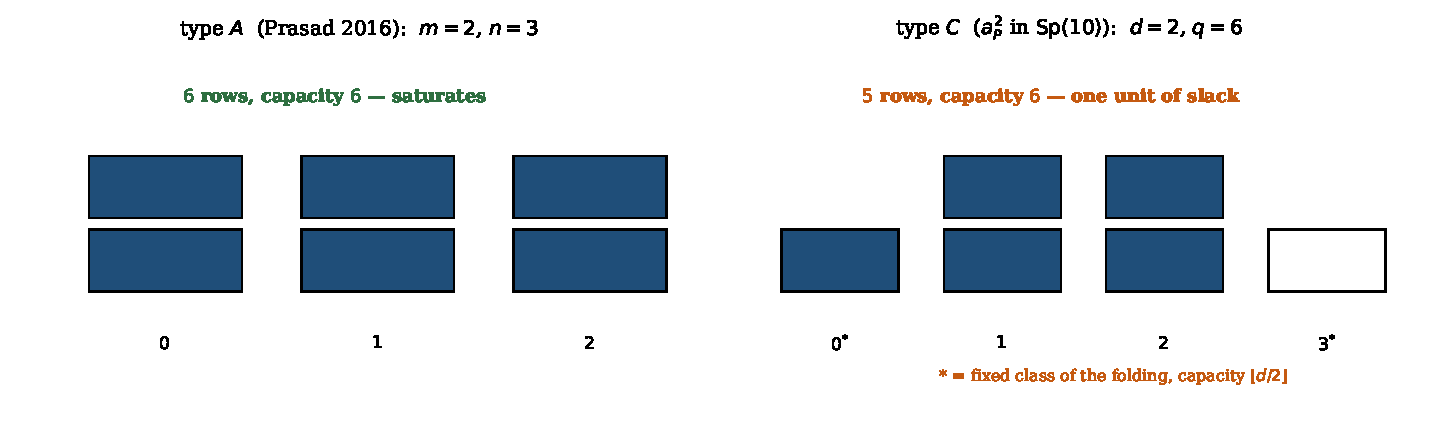
\includegraphics[width=\textwidth]{fig_capacity.pdf}
\caption{Proposition~\ref{prop:slack} drawn. Left, type $A$: the boxes fill exactly. Right, type $C$
at $a_P^2$ in $\Sp(10)$: the two starred classes are the fixed points of the involution and carry
half capacity, so five rows go into six boxes and one must stay empty. Which one \emph{is}
determined by $\lambda$: it is the unique class whose occupancy falls one below its capacity, which is
what makes $\kappa$ of Theorem~\ref{thm:dims} well defined.}
\label{fig:capacity}
\end{figure}


\section{The value, with its sign}\label{sec:valor}

\noindent\emph{So far the answer has been yes or no. When the answer is yes, what is the number?}

Write, for a vector $x$ and the positive roots of type $C$,
\[
Z_q(x)\;=\;\prod_{\substack{\alpha>0\\ q\mid(x,\alpha)}}(x,\alpha)
\qquad\text{(empty product $=1$)},
\qquad
E_{p,q}(\lambda)\;=\;\sum_{\alpha>0}\left(
\Bigl\lfloor\tfrac{p(\ell,\alpha)}{q}\Bigr\rfloor-\Bigl\lfloor\tfrac{p(\rho,\alpha)}{q}\Bigr\rfloor
\right).
\]

\begin{theorem}[the value, every power, type $C$]\label{thm:signo}
In $\Sp(2m)$, for every $k$, with $d=\gcd(k,2m+2)$, $q=(2m+2)/d$ and $p=k/d$,
\[
\boxed{\;
\chi_\lambda(a_P^{\,k})\;=\;
\begin{cases}
0, & N_q(\ell)>r_q,\\[2mm]
(-1)^{E_{p,q}(\lambda)}\,\dfrac{Z_q(\lambda+\rho)}{Z_q(\rho)}, & N_q(\ell)=r_q .
\end{cases}\;}
\]
\end{theorem}

\begin{proof}[Derivation of the sign]
Because $\sum_{\alpha>0}(\lambda,\alpha)=2(\lambda,\rho)$, the phases of \eqref{eq:ps} cancel
against its prefactor, and away from the singular parameters
\[
\chi_\lambda(g_\theta)\;=\;\prod_{\alpha>0}
\frac{\sin\bigl(\pi\theta(\ell,\alpha)\bigr)}{\sin\bigl(\pi\theta(\rho,\alpha)\bigr)} .
\]
For a positive integer $A$ with $q\nmid A$ one has
$\operatorname{sgn}\sin(\pi pA/q)=(-1)^{\lfloor pA/q\rfloor}$; and for $q\mid A$, writing
$\theta=p/q+\varepsilon$,
$\sin(\pi A\theta)=(-1)^{pA/q}\pi A\varepsilon+O(\varepsilon^3)$. When the orders of vanishing agree
--- which is \eqref{eq:crit} --- the powers of $\varepsilon$ and the factors $\pi$ cancel, each
vanishing factor leaves its own exponent, and every factor leaves its sign. Collecting them gives
$(-1)^{E_{p,q}(\lambda)}$ and the quotient $Z_q(\ell)/Z_q(\rho)$.
\end{proof}

\noindent \emph{This derivation of the sign does not use the type}, once the normalisation of
\S\ref{sec:norm} is fixed; what is used below to settle the \emph{modulus} does.

\smallskip
\noindent \textbf{The numerator $p$ drops out.} By Proposition~\ref{prop:alph} the alphabet of
$a_P^{\,k}$ depends on $d$ and $q$ only, so $a_P^{\,k}$ and $a_P^{\,d}$ have the same spectrum and
\[
\chi_\lambda(a_P^{\,k})=\chi_\lambda(a_P^{\,d}),\qquad d=\gcd(k,2m+2),
\]
whence $E_{p,q}\equiv E_{1,q}\pmod 2$ on the surviving weights. \emph{Checked: the two spectra agree
as multisets on all $32$ pairs $(m,k)$ with $m\le5$.} \ver{referee2.py} It costs nothing to keep
$p$ in the statement, and the reader may set $p=1$ throughout.

\smallskip
\noindent \textbf{And the sign needs only the residues, in order.} Writing $x_i=qh_i+r_i$ with
$0\le r_i<q$, the quotients contribute $2\sum_i(m-i+1)h_i$ to the sum of floors, which is even. What
is left is a count of three indicators. Put
\[
F_q(r_1,\dots,r_m)=\#\{i:\,2r_i\ge q\}
\;+\;\#\{i<j:\,r_i<r_j\}
\;+\;\#\{i<j:\,r_i+r_j\ge q\} .
\]
Then, on the surviving weights,
\[
\boxed{\;\operatorname{sgn}\chi_\lambda(a_P^{\,k})
=(-1)^{\,F_q(\ell\bmod q)-F_q(\rho\bmod q)}\;}
\]
\emph{Checked on all $\mathbf{11\,972}$ surviving weights, $m=2,\dots,7$, every $k$: no exception.}
\ver{referee2.py} Figure~\ref{fig:value} is what that alternation looks like. In particular the sign
is periodic modulo $qP$, since
$E_{p,q}(\lambda+q\gamma)-E_{p,q}(\lambda)=2p(\gamma,\rho)$ is even. That is the precise sense in
which the occupancies of the folded classes are not enough and the full quotients are not needed:
\emph{which} residues occur, and \emph{in what order}.

\smallskip
\noindent \emph{Where this sits.} That the character at an element of finite order is determined in
general is not new: Kumar and Prasad \cite{KP24} compute $ch(t,V(\lambda))$ for any $t\in T$ of
finite order by the Atiyah--Singer fixed-point formula on $G/P$, and derive from it the asymptotics
of $ch(t,V(n\lambda))$. Theorem~\ref{thm:signo} is a different kind of statement about a much smaller
family: an elementary closed form, in the coordinates of type $C$, for the points of one line.

\begin{keybox}
\textbf{Measured.} Theorem~\ref{thm:signo} holds --- value and sign together --- on
$\mathbf{18\,904}$ surviving weights in $\Sp(2m)$, $m=2,\dots,8$, over \emph{every} $k$, in exact
integer arithmetic: the alphabet of $a_P^{\,k}$ gives $H(z)=(1-z)^2/(1-z^q)^d$ for $d$ even and
$(1-z^2)/(1-z^q)^d$ for $d$ odd, so the character is an integer determinant and its sign is a hard
datum. Modulus alone: $18\,904$ of $18\,904$. Sign alone: $18\,904$ of $18\,904$.
\ver{signo\_Fq.py}
\end{keybox}

\begin{figure}[tbp]
\centering
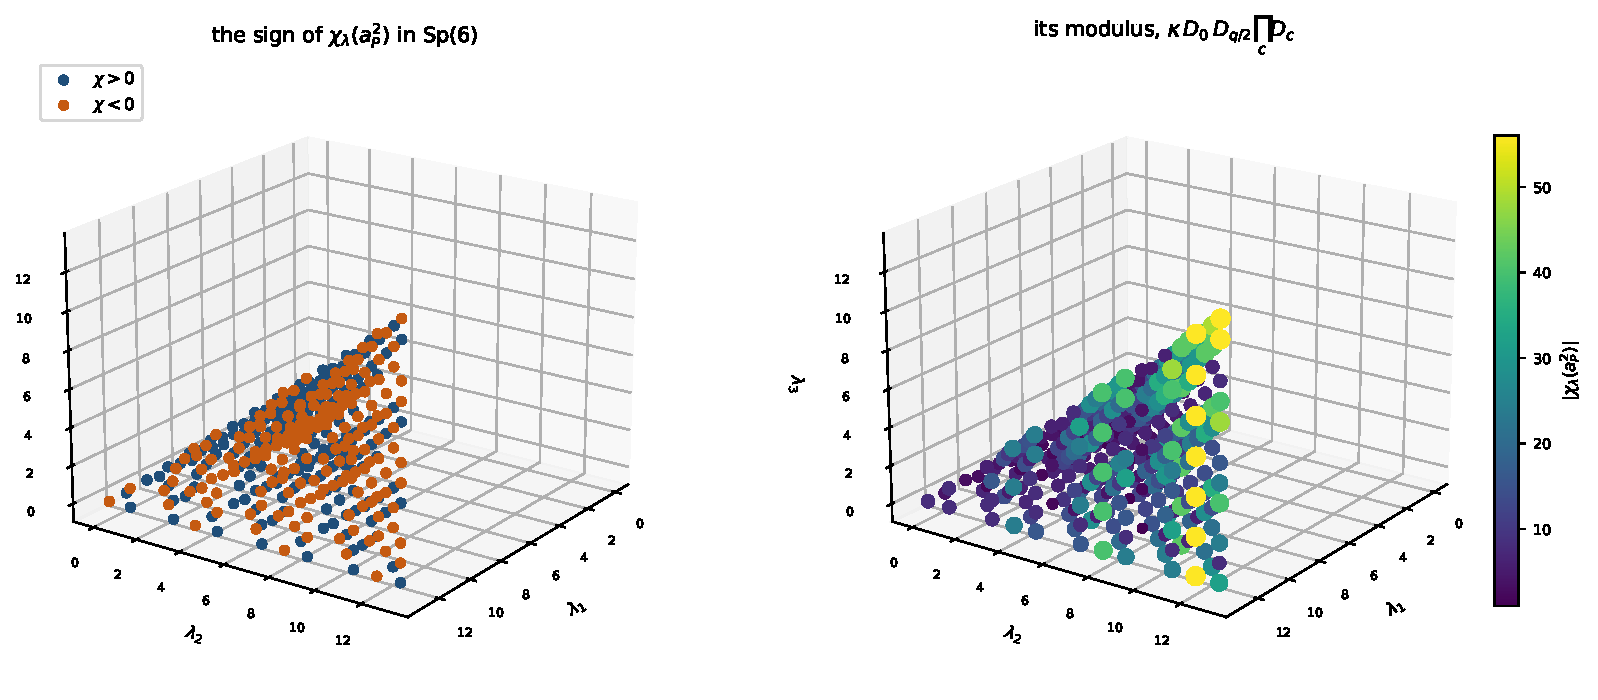
\includegraphics[width=\textwidth]{fig_value.pdf}
\caption{\textbf{The theorem, drawn.} Every dot is a surviving weight of $\Sp(6)$ at $k=2$ --- so
$d=2$, $q=4$ --- plotted at $(\lambda_1,\lambda_2,\lambda_3)$, over the box $\lambda_1\le13$; there
are $\mathbf{352}$ of them, $176$ with each sign. Left, the \emph{sign} of
Theorem~\ref{thm:signo}: it alternates in sheets. That is the picture behind the two negative
results of this section --- the sign is plainly not a function of the occupancy pattern, since
neighbouring weights with the same classes take both signs, and just as plainly not noise. Right,
the \emph{modulus}, which by Theorem~\ref{thm:dims} is $\kappa\,D_0\,D_{q/2}\prod_c D_c$; it runs
from $1$ to $\mathbf{56}$ over this box and grows along the direction in which the free class fills
up. \ver{fig\_value.py}}
\label{fig:value}
\end{figure}

\noindent \textbf{The sign does not simplify further, and it is worth saying how far that was
pushed.} Writing $(x,\alpha)=q\lfloor(x,\alpha)/q\rfloor+\bigl((x,\alpha)\bmod q\bigr)$ and using
$\sum_{\alpha>0}(x,\alpha)=2(x,\rho)$ turns $E_{p,q}$ into $2p(\lambda,\rho)/q$ corrected by the
residues; and statement (B) below says the residues of $\ell$ and of $\rho$ agree \emph{up to}
$r\leftrightarrow-r$. If they agreed on the nose the correction would vanish and the sign would be
$(-1)^{2p(\lambda,\rho)/q}$. They do not: \emph{over $11\,972$ surviving weights that candidate is
not even an integer in $6\,800$ of them, and among the rest it has the wrong parity $1\,068$ times.}
\ver{simplificaciones.py} The folding is doing real work in the sign, and the floors are the only
form found here that survives it.

\smallskip
\noindent \textbf{Why the sign was not found by looking for a parity.} Before the sine form was
written down, the sign was hunted as a $\mathrm{GF}(2)$-linear combination of fifteen natural
statistics --- the classes taking each branch of $\mp$, the parity of the quotients
$\lfloor\ell_i/q\rfloor$, of the folded rows, of $|\lambda|$, of $(\lambda,\rho)$, of the inversions
of the class word, and others. The system over $2\,582$ weights with $m\le6$ is \emph{inconsistent}:
no subset works. Nor is the sign a function of the occupancy pattern --- of the $32$ patterns that
occur, none carries a constant sign, the smallest witness being $\lambda=(1,0)$ against
$\lambda=(1,1)$ in $\Sp(4)$ at $k=2$: same classes, same modulus $2$, and characters $-2$ and $+2$.
\emph{$E_{p,q}$ is not among those fifteen and could not be: they are parities of natural
quantities, and $E_{p,q}$ is a sum of floors --- which does have a count form, $F_q$ above, but not
one of theirs.} That is what the sine form buys. \ver{sign\_k2.py}

\section{The modulus, and the lemma it rested on}\label{sec:modulo}

\noindent\emph{The sign is settled. What is left of the value is a ratio of two products of integers --- why should the factors that do \emph{not} vanish contribute nothing to it?}

The modulus half of Theorem~\ref{thm:signo} is worth stating on its own, because it holds
beyond type $C$ and because that is how it was arrived at. At $k=2$ it takes the shape of one factor
per class:

\begin{theorem}[value, $k=2$, absolute value]\label{conj:val}
For $k=2$, \textbf{and for $\lambda$ satisfying the capacities of Corollary~\ref{conj:cap}}: group
the $\ell_i$ by folded class. Then
\[
\boxed{\;|\chi_\lambda(a_P^k)| \;=\; \prod_{\text{classes}} D_c\;}
\qquad
D_c=\begin{cases}
|\ell_i\mp\ell_j|/q, & c \text{ not fixed, holding two rows } \ell_i,\ell_j,\\[2pt]
2\ell_i/q, & c \text{ fixed, holding one row},\\[2pt]
1, & \text{otherwise,}
\end{cases}
\]
the sign in $\mp$ being the one that makes the quotient an integer.
\end{theorem}

\noindent Exactly one of the two signs works: if $q$ divided both $\ell_i-\ell_j$ and
$\ell_i+\ell_j$ it would divide $2\ell_i$, and the class would be a fixed one. \emph{Checked on all
$\mathbf{27\,208}$ pairs that arise below: none ambiguous.} \ver{revision\_54\_enunciados.py}

\noindent This too follows from \eqref{eq:ps}, once one is careful about which factors vanish. At
$k=2$ one has $d=2$, $q=m+1$ and $m=q-1$: a surviving $\lambda$ leaves exactly one place free, so a
Weyl element arranges the residues of $w\ell$ as $\ZZ/q\smallsetminus\{s\}$ for some $s$; this is
legitimate in modulus because $w^{-1}\alpha$ is a positive or a negative root and
$|1-z^{-r}|=|1-z^{r}|$ for $|z|=1$, so that
$\big|\prod_{\alpha>0}(1-z^{(w\ell,\alpha)})\big|=\big|\prod_{\alpha>0}(1-z^{(\ell,\alpha)})\big|$.
The
vanishing factors of the numerator are then one per class that contributes a zero at all --- a
non-fixed class holding two rows, with exponent $|\ell_i\mp\ell_j|$, or a fixed class holding one,
with exponent $2\ell_i$; a non-fixed class holding a single row carries no root $e_i\pm e_j$ and
contributes nothing --- while in the denominator, $d$ being $2$, every vanishing exponent is exactly
$q$. Their ratio is the stated product. What remains is that the
factors which do \emph{not} vanish cancel in modulus, and that is the following, which is a fact
about roots of unity and nothing else.

\begin{proposition}\label{prop:Ms}
Write $U_s=\mu_q\smallsetminus\{\xi_q^{\,s}\}$ and let $M_s$ be the product of the \emph{absolute
values} of the non-vanishing factors of the $C_{q-1}$ Weyl product over $U_s$. Then $M_s=M_0$ for
every $s$.
\end{proposition}

\begin{proof}
Put $a=\xi_q^{\,s}$ and enumerate $U_s=\{x_1,\dots,x_{q-1}\}$ in any order. Split
$M_s=A_sB_sD_s$ with
\[
A_s=\prod_{i<j}\big|1-x_i/x_j\big|,\qquad
B_s=\prod_{\substack{i<j\\ x_ix_j\neq1}}\big|1-x_ix_j\big|,\qquad
D_s=\prod_{\substack{i\\ x_i^2\neq1}}\big|1-x_i^2\big| ,
\]
each a product over unordered pairs or over single elements, so independent of the enumeration.
Every $x_i$ has modulus one, so $A_s=\prod_{i<j}|x_i-x_j|$ is a Vandermonde. Let $P_a(X)=(X^q-1)/(X-a)$,
whose roots are exactly $U_s$; then $\prod_{x\in U_s}|P_a'(x)|=A_s^2$, while differentiating
$X^q-1=(X-a)P_a(X)$ at each root gives
$\prod_{x\in U_s}|P_a'(x)|=q^{\,q-1}\big/\prod_{x\in U_s}|x-a|$. Since
$\prod_{x\in U_s}|a-x|=\big|(X^q-1)'\big|_{X=a}=q$, this yields
\[
A_s^2=q^{\,q-2},\qquad\text{that is}\qquad A_s=q^{(q-2)/2},
\]
independently of $s$. Now take the \emph{ordered} product
$C_s=\prod_{i,j:\ x_ix_j\neq1}|1-x_ix_j|$ over all ordered pairs, so that $C_s=B_s^2D_s$. Over $\mu_q$, every $x$ has
$\prod_{y\neq x^{-1}}|1-xy|=q$, and removing $a$ from the outer and the inner range gives
\[
C_s=q^{\,q-2}\big|1-a^2\big|\ \ (a^2\neq1),\qquad C_s=q^{\,q-2}\ \ (a^2=1),
\]
while with $D=\prod_{x\in\mu_q,\,x^2\neq1}|1-x^2|$ the same removal gives $D_s=D/|1-a^2|$,
respectively $D_s=D$. In both cases the extra factor cancels:
\[
C_sD_s=q^{\,q-2}D ,
\]
which is independent of $s$. Hence so is $(B_sD_s)^2=C_sD_s$, hence so is $B_sD_s$; with $A_s$ that
gives $M_s=M_0$.
\end{proof}

\noindent \emph{Every step of that argument was checked for $q=3,\dots,11$ and every $s$, to
$3\cdot10^{-15}$ --- together with a decoy: the same product read as a complex number, without the
absolute values, does depend on $s$ in $6$ of $6$ cases, which is why the statement is about moduli.
For the record $D=q$ for $q$ odd and $(q/2)^2$ for $q$ even, though independence needs no such
value.} \ver{revision\_49\_prueba\_Ms.py}

\begin{theorem}[the absolute value, any $k$ --- modulo Lemma~\ref{lem:unit}]\label{thm:valgen}
Let $\ell=\lambda+\rho$ and suppose $\chi_\lambda(a_P^k)\neq0$. Then
\[
\boxed{\;\bigl|\chi_\lambda(a_P^{\,k})\bigr|\;=\;
\frac{\prod_{\alpha>0,\ q\mid(\ell,\alpha)}(\ell,\alpha)}
     {\prod_{\alpha>0,\ q\mid(\rho,\alpha)}(\rho,\alpha)}\;}
\]
\end{theorem}

\begin{proof}[Derivation]
Put $z=\xi_q(1+\varepsilon)$. If $q\mid a$ then $z^a=(1+\varepsilon)^a$, so
$1-z^a=-a\varepsilon+O(\varepsilon^2)$: every vanishing factor contributes its own exponent, and one
power of $\varepsilon$. By \eqref{eq:crit} the numerator and the denominator of \eqref{eq:ps} carry
the same number $r_q$ of vanishing factors, so the powers of $\varepsilon$ cancel and their ratio
tends to the ratio of the products of the exponents --- with no pairing of roots required, which is
the point. Hence
\begin{equation}\label{eq:split}
\chi_\lambda(a_P^{\,k})\;=\;\xi_q^{-(\lambda,\rho)}\cdot
\frac{\prod_{q\mid(\ell,\alpha)}(\ell,\alpha)}{\prod_{q\mid(\rho,\alpha)}(\rho,\alpha)}\cdot U,
\qquad
U=\frac{\prod_{q\nmid(\ell,\alpha)}\bigl(1-\xi_q^{(\ell,\alpha)}\bigr)}
        {\prod_{q\nmid(\rho,\alpha)}\bigl(1-\xi_q^{(\rho,\alpha)}\bigr)} .
\end{equation}
For $\lambda$ dominant every $(\ell,\alpha)$ and every $(\rho,\alpha)$ with $\alpha>0$ is a positive
integer, so the middle factor is a positive rational. The theorem is therefore exactly the statement
$|U|=1$.
\end{proof}

\begin{lemma}[the unit]\label{lem:unit}
The factor $U$ of \eqref{eq:split} has modulus $1$.
\end{lemma}

\noindent \textbf{At $d=2$ this lemma is Proposition~\ref{prop:Ms}}, and there every vanishing
$(\rho,\alpha)$ equals $q$, so the denominator of Theorem~\ref{thm:valgen} is $q^{\,r_q}$ and the
statement becomes Theorem~\ref{conj:val} in the coordinates of type $C$. For $d\ge3$ I have not
proved it, and I want to be exact about what that leaves: \emph{the value is no longer a limit to be
evaluated. It is a finite statement about roots of unity} --- that two explicit products of
$1-\xi_q^{\,r}$ have the same modulus --- \emph{with no character, no branching and no
representation theory left in it.}

\smallskip
\noindent More than that: it is a congruence, and it can be proved outright.

\section{The residue lemma, and what it turned out to see}\label{sec:res}

\noindent Lemma~\ref{lem:unit} is the one step the modulus rested on, and it is not really a
statement about products. Since $|1-\xi_q^{\,r}|$ depends only on $r$ modulo $q$ and
$|1-\xi_q^{\,r}|=|1-\xi_q^{-r}|$, it follows from an equality of two multisets of residues.
Written that way it says more than the step it was made for.

\begin{proposition}[the residue lemma]\label{prop:res}
Work in $\ZZ[X]/(X^q-1)$. For $x=(x_1,\dots,x_m)$ put
\[
P_x(X)=\sum_{i=1}^{m}\bigl(X^{x_i}+X^{-x_i}\bigr),
\qquad
\mathscr{R}_x(X)=\sum_{\alpha\in\Phi(C_m)}X^{(x,\alpha)} .
\]
Then
\begin{equation}\label{eq:res}
\boxed{\;\mathscr{R}_x(X)\;=\;\frac{P_x(X)^2+P_x(X^2)}{2}\;-\;m\;}
\end{equation}
and, for every $\lambda$ satisfying the capacities of Corollary~\ref{conj:cap},
$\mathscr{R}_{\lambda+\rho}=\mathscr{R}_\rho$.
\end{proposition}

\begin{proof}
Expanding $P_x(X)^2$ collects $X^{\pm x_i\pm x_j}$ over all ordered pairs. The off-diagonal terms
give each root $\pm e_i\pm e_j$ twice; the diagonal terms give $X^{\pm2x_i}$ once each and $2m$
copies of $X^0$; and $P_x(X^2)$ supplies the second copy of each $X^{\pm2x_i}$. Halving therefore
leaves every root of $C_m$ exactly once, together with $m$ copies of $X^0$, and subtracting $m$
removes those. That is \eqref{eq:res}.

For the second claim write $T_q(X)=1+X+\dots+X^{q-1}$, so that $T_q(X)\,X^{c}=T_q(X)$ for every $c$.
If $d$ is odd the capacities are saturated, the folded occupancies of $\ell$ are those of $\rho$, and
$P_\ell=P_\rho$ outright. If $d$ is even, one class $c$ falls a single unit below its capacity, and
\[
P_\ell(X)=d\,T_q(X)-X^{c}-X^{-c},\qquad P_\rho(X)=d\,T_q(X)-2 ,
\]
so that $P_\ell(X)^2-P_\rho(X)^2=X^{2c}+X^{-2c}-2$ while
$P_\ell(X^2)-P_\rho(X^2)=-X^{2c}-X^{-2c}+2$. The two corrections cancel in \eqref{eq:res}, and
$\mathscr{R}_\ell=\mathscr{R}_\rho$.
\end{proof}

\begin{keybox}
\textbf{What \eqref{eq:res} really says, and it does not mention the type.} The weights of the
adjoint representation are the roots together with $\mathrm{rank}$ copies of $0$, so for
\emph{every} simple $G$ and every $x$,
\begin{equation}\label{eq:adj}
\boxed{\;\mathscr{R}_x(X)\;=\;\operatorname{ch}\mathfrak g\,(x)\;-\;\mathrm{rank}\;}
\end{equation}
Equation~\eqref{eq:res} is the instance of \eqref{eq:adj} in type $C$, where the adjoint is
$\mathrm{Sym}^2$ of the standard representation and $\operatorname{ch}\mathrm{Sym}^2$ is
$\tfrac12\bigl(P_x(X)^2+P_x(X^2)\bigr)$. In the classical orthogonal types the adjoint is
$\Lambda^2$ of the natural representation instead, and the same line gives
$\tfrac12\bigl(A_x(X)^2-A_x(X^2)\bigr)-m$ --- with $A_x=P_x+1$ in type $B$, where the natural
representation has $2m+1$ weights and one of them is $0$, and $A_x=P_x$ in type $D$, where it
has $2m$ and none. The minus sign is $\Lambda^2$ against $\mathrm{Sym}^2$, and nothing else.
\emph{Checked as an identity of Laurent polynomials on $7\,200$ random integer vectors, $C_2$
to $C_7$, $B_2$ to $B_7$ and $D_2$ to $D_7$: no discrepancy. The one-line control is $X=1$:
$D_4$ has $24$ roots, and reading its natural representation with a zero weight would give
$32$.} \ver{simplifica2.py, tipo\_D.py}

\smallskip
\textbf{And then the second claim is an invariance.} In $\ZZ[X]/(X^q-1)$ the quantity
$\mathscr{R}_x$ depends on $x$ only through the residues $(x,\alpha)\bmod q$, so it is fixed by the
Weyl group $W$, which permutes $\Phi$; by the translations $q Q^\vee$, since $(x+q\gamma,\alpha)
\equiv(x,\alpha)$; and by the kernel of $P/qP\to\operatorname{Hom}(Q,\ZZ/q)$, which in type $C$ is
$\{0,\tfrac q2(1,\dots,1)\}$ for $q$ even. Write $\widehat W_q^{+}$ for the group they generate.
Then
\[
\ell\in \widehat W_q^{+}\!\cdot\rho \quad\Longrightarrow\quad \mathscr{R}_\ell=\mathscr{R}_\rho ,
\]
with no computation and in any type. \emph{Measured: the orbit is contained in the surviving
weights with $\mathbf{0}$ false positives over $1\,134$ weights, and exhausts them exactly when $d$
is odd or $q=2$; for $d$ even with $q\ge3$ the survivors are strictly more, which is the free place,
and that is the case the displayed cancellation above settles.} \ver{orbita.py}
\end{keybox}

\noindent Grouping each root with its negative turns that equality into

\begin{keybox}
\textbf{(B)} \quad For every surviving $\lambda$, the two multisets
\[
\bigl\{\,(\ell,\alpha)\bmod q \;:\; \alpha>0,\; q\nmid(\ell,\alpha)\,\bigr\}
\qquad\text{and}\qquad
\bigl\{\,(\rho,\alpha)\bmod q \;:\; \alpha>0,\; q\nmid(\rho,\alpha)\,\bigr\}
\]
coincide once $r$ and $-r$ are identified.
\end{keybox}

\noindent and (B) pairs the surviving factors of \eqref{eq:split} one to one with factors of equal
modulus. \textbf{So Lemma~\ref{lem:unit} is proved, and with it Theorem~\ref{thm:valgen} in type
$C$}: nothing in this section rests on a measurement any more. The converse needs no experiment
either --- equal multisets of non-zero residues have equal cardinality, so the counts of zero
residues agree, which is \eqref{eq:crit}.

\smallskip
\noindent What the proof also explains is why the obvious route fails. The stronger condition
$\ell\equiv w(\rho)\pmod q$ for some $w\in W$ --- equality of the folded classes of $\ell$ and of
$\rho$ themselves --- is sufficient and gives (B) at once, and it is what happens when $d$ is odd.
For $d$ even it is false: the smallest witness is $\Sp(4)$ at $k=2$ with $\lambda=(1,0)$, where
$\ell=(3,1)$ and $\rho=(2,1)$ have folded classes $\{0,1\}$ against $\{1,1\}$, while the
non-vanishing exponents $\{2,4,2\}$ and $\{1,4,2\}$ have residues that agree once $r$ and $-r$ are
identified. \textbf{The pairing is between the surviving factors, not between $\ell$ and $\rho$},
and \eqref{eq:res} is what makes that visible.

\emph{Checked all the same, because an identity of this shape is easy to write with a sign wrong:
\eqref{eq:res} on $\mathbf{48\,669}$ vectors, and $\mathscr{R}_\ell=\mathscr{R}_\rho$ on all
$\mathbf{11\,972}$ surviving weights of $\Sp(2m)$ with $m=2,\dots,7$ and every $k$ --- no exception.}
\ver{referee2.py}

\begin{keybox}
\textbf{Measured, and the decoys say the measurement discriminates.} Over $\mathbf{7\,778}$
surviving weights in $\Sp(2m)$ with $m=2,\dots,8$ and every $k$ giving $d\ge3$ --- that is
$d=3,4,5,6,7,8,9$ --- Theorem~\ref{thm:valgen} holds \textbf{without one exception}, in exact integer
arithmetic: at $k$ arbitrary the alphabet gives $H(z)=(1-z)^2/(1-z^q)^d$ for $d$ even and
$(1-z^2)/(1-z^q)^d$ for $d$ odd, so the character is an integer determinant. Three decoys over the
same weights: the same formula \emph{without the denominator} agrees $0$ times; read on
\emph{coroots} instead of roots, $2\,084$ times; taken over \emph{all} the positive roots instead of
only the vanishing ones, $17$ times. And \eqref{eq:crit} itself, checked in passing on all
$\mathbf{15\,477}$ weights of that run, holds without exception.
\end{keybox}
\ver{value\_general\_d.py}

\noindent The denominator is the case $s=0$ of the same product: at $d=2$ the half-sum is
$\rho=(q-1,q-2,\dots,1)$, whose residues are $\ZZ/q\smallsetminus\{0\}$, so its non-vanishing part
is $M_0$. Proposition~\ref{prop:Ms} therefore says numerator and denominator have the same modulus
outside the vanishing factors, and with $|z^{-(\lambda,\rho)}|=1$ that closes the absolute value at
$d=2$. \textbf{Both of the things this paragraph once left open are settled above}: the sign by
Theorem~\ref{thm:signo}, and $d\ge3$ by Theorem~\ref{thm:valgen} together with the box below, which
proves Lemma~\ref{lem:unit} in type $C$.

I state it in coordinates because that is the form the proof gives, and because the tidier
form does not survive checking. It is tempting to write the same thing as
$\prod_{\alpha\in R_P(q)^+}(\ell,\alpha)/(\rho_P,\alpha)$, a Weyl dimension
for the centralizer, with $R_P(q)=\{\alpha : q\mid(\rho,\alpha)\}$. Two things go wrong.
First, $(\rho_P,\alpha)$ --- $\rho_P$ being the half-sum of $R_P(q)^+$ --- is never $q$;
it takes the values $1$, or $1,2$, or $1,2,3$ according to the case, so the denominator above is not
$(\rho_P,\alpha)$ but $q$. Second, $(\rho,\alpha)=q$ for \emph{every}
$\alpha\in R_P(q)$ only when $d=2$ --- which is the case $k=2$ proved here; at $d=4$ the values
are $\{3,6,9\}$ and $\{4,8,12\}$. So the Weyl-dimension reading is a description of the $k=2$
case, not a proved general form, and the $\ell$ appearing in it would still have to be moved into
the right chamber by a Weyl element I have not identified. \ver{socratico\_zonas\_oscuras.py}

\noindent That was measured before it was proved, and I have kept the measurement because it is what
would have caught me: $\mathbf{4632}$ weights over the same box, no exception, while the control
that drops the fixed-class factor falls to between $42\%$ and $77\%$ depending on the rank. \ver{aP\_potencias.py}

\noindent Figure~\ref{fig:union3d} draws what is at stake in passing from $a_P$ to its powers, and
it is the reason this note is about the powers at all: at $a_P$ itself every surviving value is
$\pm1$ --- Kostant's theorem --- while one power later, at the same rank, they run to $72$.

\begin{figure}[tbp]
\centering
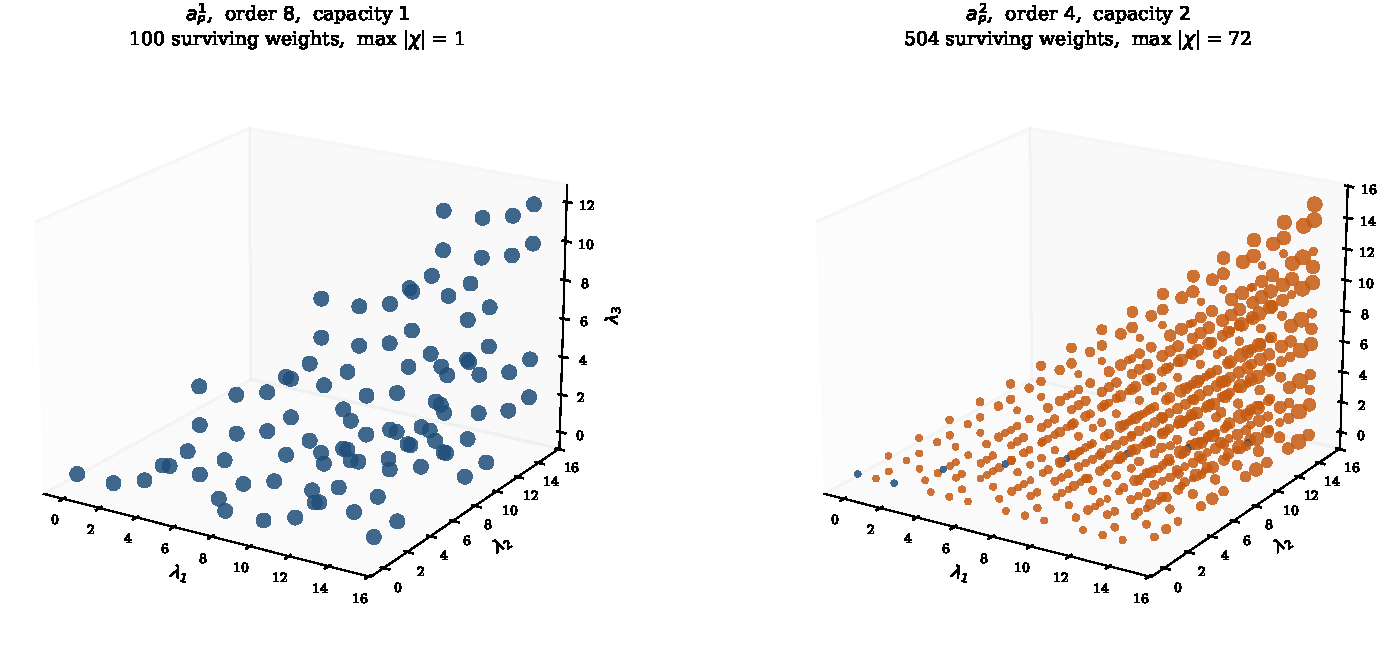
\includegraphics[width=\textwidth]{fig_union3d.pdf}
\caption{Why the powers are where the content is, and $a_P$ itself is not. Left: capacity one,
$100$ survivors, every value $\pm1$. Right: capacity two, $504$ survivors, values up to $72$. Both
in $\Sp(6)$ over the box $0\le\lambda_3\le\lambda_2\le\lambda_1\le15$. Dot
size is $|\chi|$ and blue marks $|\chi|=1$, so the blue points on the right are the ones that behave
as if they were still at $a_P$. At $a_P$ every block of the centralizer is a torus and every
dimension is $1$ --- which is exactly the case $m=1$ of \cite{Prasad16b}.}
\label{fig:union3d}
\end{figure}



\begin{keybox}
\textbf{And in type $C$ the lemma is proved, so Theorem~\ref{thm:signo} stands on its own.} The
argument of Proposition~\ref{prop:Ms} generalises from $d=2$ to every multiplicity, with one
definition added: for a multiset $U$ with repetitions the Vandermonde part has to be the
\emph{reduced} product
$A_{\mathrm{red}}(U)=\prod_{i<j,\ x_i\neq x_j}|1-x_i/x_j|$, since $s\cdot\mu_q$ repeats each
root $s$ times and the unreduced product is zero for $s>1$. With $A_{\mathrm{red}}$ in place of $A$
throughout, the deletion argument goes through unchanged. For $d$ odd the
capacities are saturated, the occupancies of all folded classes are those of $\rho$, and signs and
permutations of the coordinates carry one set of residues onto the other. For $d=2s$ one place is
free, and the multiset of the $m$ quantities $\xi_q^{(w\ell)_i}$ can be written as
$U_a=s\cdot\mu_q-\{a\}$ with $a\in\mu_q$, that of $\rho$ being $U_1$. Writing $M(U)$ for the reduced
product, $M(U)^2=A(U)^2C(U)D(U)$ in the notation of the proof above, and deleting one copy of $a$
from $\mathcal B=s\cdot\mu_q$ gives, by $\prod_{y\in\mu_q,\,y\neq a^{-1}}|1-ay|=q$,
\[
A(U_a)=\frac{A(\mathcal B)}{q^{s}},\qquad
C(U_a)=\frac{C(\mathcal B)}{q^{2s}}F(a),\qquad
D(U_a)=\frac{D(\mathcal B)}{F(a)},
\]
with $F(a)=|1-a^2|$ when $a^2\neq1$ and $F(a)=1$ otherwise, so that
$M(U_a)^2=A(\mathcal B)^2C(\mathcal B)D(\mathcal B)/q^{4s}$, independent of $a$. That the vanishing
exponents of the denominator run through $q,2q,\dots$ rather than all being $q$ is not an
obstruction: they are collected in $Z_q(\rho)$.
\end{keybox}

\subsection*{What the difference of two residue histograms is}

\noindent Proposition~\ref{prop:res} says $\mathscr{R}_{\lambda+\rho}=\mathscr{R}_\rho$ when the
capacities of Corollary~\ref{conj:cap} are met exactly. When they are not, the difference is not
noise: it is the residue histogram of \emph{another root system}, of bounded rank.

\begin{proposition}[the difference is another group's]\label{prop:resid}
Let $\ell=\lambda+\rho$ satisfy $N_q(\ell)=N_q(\rho)$, write $m=uq+v$ with $0\le v<q$ and
$a=\lfloor(q-1)/2\rfloor$, and let $S=\{s_1>\dots>s_r\}$ be the folded classes at which the
occupancy departs from the flat profile: those carrying a surplus row when $v\le a$, where $r=v$;
those short of one when $v>a$, where $r=q-v$. With $T_q=\sum_{k=0}^{q-1}X^k$ and
$C_S=\sum_{c\in S}(X^c+X^{-c})$,
\[
P_\ell=\begin{cases}2u\,T_q+C_S, & v\le a,\\[1mm] 2(u+1)\,T_q-C_S, & v>a,\end{cases}
\]
and, writing $H=C_r$ when $v\le a$ and $H=D_r$ when $v>a$, with $\rho_H$ its half-sum and
$\eta_i=s_i-(\rho_H)_i$,
\[
\boxed{\;\mathscr{R}_{\lambda+\rho}-\mathscr{R}_{\rho}
\;=\;\mathscr{R}^{H}_{\eta+\rho_H}-\mathscr{R}^{H}_{\rho_H}\;}
\]
\end{proposition}

\begin{proof}
The two shapes of $P_\ell$ are the minimal profiles of the proof of Theorem~\ref{thm:cuenta},
which is stated for every $q$: below the
half-way point the flat profile is $2u$ per non-fixed class and $u$ per fixed one, and $v$ classes
carry one row more; above it the flat profile is one higher and $q-v$ classes carry one row less.
In $\ZZ[X]/(X^q-1)$ one has $T_q^2=q\,T_q$ and $T_qC_S=2|S|\,T_q$. Since $\rho$ has the same $u$
and $|S_0|=|S|$, every term carrying $T_q$ is the same for $\ell$ and for $\rho$, and drops out of
the difference; what is left is
\[
\mathscr{R}_{\lambda+\rho}-\mathscr{R}_\rho
=\frac{\bigl(C_S^2\pm C_S(X^2)\bigr)-\bigl(C_{S_0}^2\pm C_{S_0}(X^2)\bigr)}{2},
\]
the sign being the one with which $C_S$ enters $P_\ell$: squaring does not see it, $X\mapsto X^2$
does. Read \eqref{eq:res} in rank $r$: the upper sign is $\mathscr{R}^{C_r}$ and the lower one
$\mathscr{R}^{D_r}$, since $P(X^2)$ is exactly the long roots $2e_i$ and $D_r$ has none. Finally
$S_0$ --- the departure set of $\rho$ itself --- is $\rho_H$, so $C_{S_0}=P_{\rho_H}$ and
$C_S=P_{\eta+\rho_H}$.
\end{proof}

\noindent \emph{Checked on $\mathbf{3\,729}$ surviving weights with $m\le7$ and $q\le14$: the
identity holds without exception, and so does the intermediate shape of $P_\ell$ on the same
$3\,729$; the assignment of type is never crossed, $v\le a$ giving $C_r$ in $1\,365$ of them and
$v>a$ giving $D_r$ in $2\,364$. Three decoys --- swapping the type, shifting $\eta$ by one, and
omitting $\rho_H$ --- break $447$, $407$ and $717$ of $1\,103$.}
\ver{residual\_histogramas.py}

\begin{keybox}
\textbf{And that is what the corrector is, measured.} Write $\mathcal D(\lambda,q)$ for the product
of dimensions of \S\ref{sec:dims} and $\kappa_q(\lambda)$ for the constant there. \emph{Over
$\mathbf{1\,814}$ surviving weights with $m\le6$ and $q\le12$ --- every $q$, not only those
dividing $t$ ---}
\[
\bigl|\chi_\lambda(g_{1/q})\bigr|
=\kappa_q(\lambda)\,\mathcal D(\lambda,q)\,\chi^{H}_{\eta}\bigl(h^{H}_{1/q}\bigr),
\]
\emph{without exception, where $h^H_{1/q}$ is the point of the $\rho_H$-line of $H$ at the same
denominator.} The residual point is regular --- every root value of $H$ stays strictly between $0$
and $q$ --- so nothing here has been moved to a second singular limit. \emph{Four decoys break it:
shifting $\eta$, swapping the type, forcing $\kappa=1$, and taking the residual to be $1$ --- which
is the older statement --- fail $390$, $386$, $371$ and $355$ of $1\,145$.} Outside the four
families the residual is where the irrationality goes: the integer factor still splits off.
\emph{This is a measurement, not a theorem: what is proved above is the identity of histograms, and
the step from it to the absolute value and the sign is not.}
\ver{residual\_factorizacion.py}
\end{keybox}

\section{A factorisation into dimensions}\label{sec:dims}

\noindent\emph{The value came out as a ratio of two products of integers, and the ratio is always a whole number. Is it counting something?}

The quotient $Z_q(\ell)/Z_q(\rho)$ can be read as a product of dimensions, one per folded class. Before
that is done, the prior art has to be put where it belongs.

\begin{keybox}
\textbf{Factorising a twisted classical character into characters of smaller classical groups,
indexed by the $t$-quotient, is Ayyer--Kumari.} Their Theorem~2.11 of \cite{AK22} does exactly that
for $\mathrm{sp}_\lambda(X,\omega_tX,\dots,\omega_t^{t-1}X)$ --- the \emph{undeleted} alphabet ---
and the partitions indexing the factors are the components of $\mathrm{quo}_t(\lambda)$, with $Sp$
and $SO$ appearing as here. What is done below is the same shape for the alphabet of
Proposition~\ref{prop:alph}, which is that one \emph{short of two letters}, specialised at
$x_i=1$ so that the characters become dimensions. The two deleted letters do \emph{not} produce the
fixed classes --- those are the solutions of $2c\equiv0\pmod q$, and they exist for the folding
alone, one when $q$ is odd and two when it is even --- but they do change the \emph{occupancies} of
those classes, and with them the factor $\kappa$. The pattern is theirs; the deletion, the specialisation and
$\kappa$ are what is added.
\end{keybox}

Let $\lambda$ satisfy the capacities. For a non-fixed class $c$ holding $n$ rows, orient each row by
a sign so that $\varepsilon_i\ell_i\equiv c\pmod q$, sort the integers
$y_i=(\varepsilon_i\ell_i-c)/q$ in decreasing order, and put
$\nu^{(c)}_i=y_i-y_n-(n-i)$. For the fixed class $0$ with rows $\ell_1>\dots>\ell_n$ put
$\nu^{(0)}_i=\ell_i/q-(n-i+1)$; and when $q$ is even, for the fixed class $q/2$,
$\nu^{(q/2)}_i=\ell_i/q-(n-i+\tfrac12)$. These are partitions, and empty classes contribute $1$.

\begin{theorem}[the modulus, factored]\label{thm:dims}
With $D_c=\dim V^{GL_n}_{\nu^{(c)}}$ on a non-fixed class, $D_0=\dim V^{Sp_{2n}}_{\nu^{(0)}}$ and
$D_{q/2}=\dim V^{SO_{2n+1}}_{\nu^{(q/2)}}$,
\[
\boxed{\;
\bigl|\chi_\lambda(a_P^{\,k})\bigr|\;=\;\kappa(\lambda)\,D_0\,D_{q/2}
\prod_{c\ \text{not fixed}} D_c \;}
\]
omitting $D_{q/2}$ when $q$ is odd, where $\kappa(\lambda)=1$ if $d$ is odd, $1$ if $d$ is even and
the free place lies in the class $0$, and $2$ otherwise.
\end{theorem}

\begin{keybox}
\textbf{None of the construction used $q\mid t$.} The partitions $\nu^{(c)}$ are built from the
folded classes of $\ell$ and the ladders of the three families, and nothing in that recipe knows
which denominator it is standing at. The same is true of the quotient it computes:
\emph{over the $\mathbf{2\,186}$ surviving weights of $\Sp(2m)$ with $m=2,\dots,5$ at every
$q=2,\dots,12$ --- and not only at the $q$ dividing $2m+2$ ---}
\[
\frac{Z_q(\lambda+\rho)}{Z_q(\rho)}\;=\;\kappa_q(\lambda)\,D(\lambda,q),
\qquad \kappa_q(\lambda)\in\{1,2\},
\]
\emph{without exception, with $\kappa_q=1$ in $1518$ of them and $2$ in $668$.} What is proved below
is the case $q\mid t$; the rest is measurement, and it says the theorem is narrower than its
argument. Theorem~\ref{thm:clasif} says which of those denominators are the ones where the character
itself is a whole number. \ver{teorema\_II.py}
\end{keybox}

\noindent The check is on the denominators of the dimension formulas. After the powers of $q$ come
out, the block constants are $V_n=\prod_{j<n}j!$ for $GL_n$, $C_n=2^n\prod_{j\le n}(2j-1)!$ for the
class $0$ and $B_n=\prod_{j\le n}(2j-1)!$ for the class $q/2$; for $d$ odd they cancel against the
denominator, and for $d=2s$ moving the free place out of the class $0$ produces exactly the factor
$2$, since $C_s/C_{s-1}=2(2s-1)!$ while $V_{2s}/V_{2s-1}=B_s/B_{s-1}=(2s-1)!$. \emph{Measured on
$\mathbf{11\,972}$ surviving weights, $m=2,\dots,7$, every $k$: no exception.}
\ver{dims\_recuento.py}

\noindent The free place is determined by $\lambda$ --- it is the unique class whose occupancy falls
one below its capacity --- so $\kappa$ is well defined. \emph{Checked on $10\,230$ surviving weights
with $d$ even: in every one there is exactly one such class.} \ver{signo\_Fq.py}

\begin{keybox}
\textbf{When $d$ is odd the group does not depend on $\lambda$ at all.} The capacities are then
saturated, so every surviving weight has the \emph{same} occupancy profile --- and it is the profile
of $\rho$ itself. \emph{Measured on $\mathbf{7\,166}$ surviving weights with $d$ odd,
$m=2,\dots,9$: not one has a different profile.} \ver{simplificaciones.py} So for odd $d$ the
product $\prod_c D_c$ is a dimension for one fixed group, the same for every $\lambda$, and
$\lambda$ only chooses the highest weight inside it: Theorem~\ref{thm:dims} is a decomposition
indexed by blocks rather than a numerical coincidence. When $d$ is even exactly one block loses a
row, and $\kappa$ records which.

\smallskip
\textbf{And the group carries a fingerprint.} The blocks are $GL_{n}$ on the non-fixed classes,
$Sp_{2n}$ on the class $0$ --- and $SO_{2n+1}$ on the class $q/2$. Odd orthogonal against symplectic
is the Langlands dual pair, and the two counts of \cite{NPP25} are read there as dimensions of
centralisers in the \emph{dual} group. That is a strong hint about which group these dimensions
belong to, and it is what makes the first question of \S\ref{sec:preguntas} worth asking rather than
merely open.

\smallskip
\textbf{And the fingerprint is older than the element.} Lecouvey \cite[\S3.2.2]{Lec07a} takes the
\emph{full} alphabet, folds the classes of $\mu+\rho$ modulo $\ell$ exactly as they are folded here,
and the three types are already written on his blocks: the class $0$ carries
$\prod_{r\le s}(1-x_rx_s)$, which is type $C$; the folded pairs carry type $A$; and for even $\ell$
the class $\ell/2$ carries a Vandermonde of type $B_{r_p}$, of half sum
$(\tfrac12,\dots,r_p-\tfrac12)$. For odd $\ell$ he closes it as an identity --- a character of the
Levi $Sp\times GL\times\cdots\times GL$ \cite[Thm.~3.2.3]{Lec07a}. \emph{For even $\ell$ he proves
that one cannot:} those type-$B$ roots are not in the root lattice of $\Sp_{2n}$, and the
coefficients then \textbf{are not branching coefficients and their signs alternate}
\cite[Prop.~3.2.5]{Lec07a}.

\smallskip
\textbf{What is different here, and what is not.} His Proposition~3.2.5 is about the
\emph{coefficients} of a decomposition, not about whether a value factorises: at even order and on
the full alphabet the value does factorise, with the odd orthogonal factor, by Theorem~2.11(2) of
\cite{AK22}. So nothing here overcomes that proposition, and the even case needs no rescuing. What
is different is the alphabet: it is his short of two letters (Proposition~\ref{prop:alph}), and the
deletion is what moves the profiles and puts the constant $\kappa\in\{1,2\}$ in front of the
dimensions.
\end{keybox}

\begin{keybox}
\textbf{An example, since the recipe has several steps.} In $\Sp(10)$ with $k=4$, so $d=4$, $q=3$
and $p=1$, take $\lambda=(3,2,1,0,0)$. Then $\ell=(8,6,4,2,1)$, the quotient $Z_3(\ell)/Z_3(\rho)$ is
$8$ and $E_{1,3}(\lambda)=17$, so $\chi_\lambda(a_P^4)=-8$; and the factorisation reads
$\dim V^{GL_4}_{(1,1,1,0)}=4$ times $\dim V^{Sp_2}_{(1)}=2$.
\end{keybox}

\noindent A caution the form invites: these are dimensions of representations of groups built out of
the \emph{quotient} data of each class, not of the centraliser of $a_P^{\,k}$ itself. Identifying
them with anything on that side needs an argument this note does not have --- see
\S\ref{sec:preguntas}.

\section{How many characters survive}\label{sec:cuenta}

\noindent\emph{We can now say which weights survive and what they are worth. How many are there?}

The criterion is a condition on a point and an arrangement of walls modulo $q$, so counting the
survivors is a question with no representation theory left in it. Write
$S_X(q)=\#\{x\in P/qP: N_q(x)=r_q\}$.


\begin{keybox}
\[
S_X(q)\;=\;\prod_{i=1}^{n}\,(q-m_i),\qquad m_i \text{ the exponents of } W,
\]
\textbf{exactly when} $r_q=0$ \textbf{and} $q$ is coprime to the bad primes of $X$ --- none in type
$A$, $2$ in $B$, $C$ and $D$, and $2$ and $3$ in $G_2$, $F_4$ and $E_6$. All four cells of that
equivalence, over the $298$ pairs (type, $q$) measured: $\mathbf{138}$ where both sides hold,
$\mathbf{160}$ where neither does, and \textbf{none} in either off-diagonal cell. The decoy
$\prod_i(q-i)$ --- which coincides with the exponents in type $A$ and nowhere else --- fails $221$
times, so the agreement is with the exponents and not with the rank.
\ver{survivors\_law.py}
\end{keybox}

\noindent The right-hand side is the familiar product; I claim nothing new for it, and this note does
not need it. What the measurement buys is the \emph{boundary}, and the boundary is where the subject
of this note lives. The order of $a_P$ in $\Sp(2m)$ is $2m+2$, which is \emph{always even}, and $2$
is a bad prime in type $C$. So the classical count never applies at Kostant's second element, nor at
any of its powers --- not by a small correction but by a wide margin: at $q=6$ in $C_2$, which is
$a_P$ itself, eight weights survive where the product would give fifteen
(Figure~\ref{fig:walls}). \emph{Test:} in rank two the even case is visibly $S(q)=S(q-1)$ for
$B_2$ and $C_2$; it survives to rank three in $C_3$ and \emph{breaks in $B_3$}, where $r_q=0$
and the two counts still differ --- so it is not the regularity of $\rho$ that governs it. The
first thing to find is what replaces it. \emph{What it would buy:} a generating function in $q$ for how much of the
representation ring survives at a torsion element, on the side of the two Kostant elements where
there is currently no formula at all.
\ver{survivors\_quasipoly.py, survivors\_law.py}

\begin{figure}[tbp]
\centering
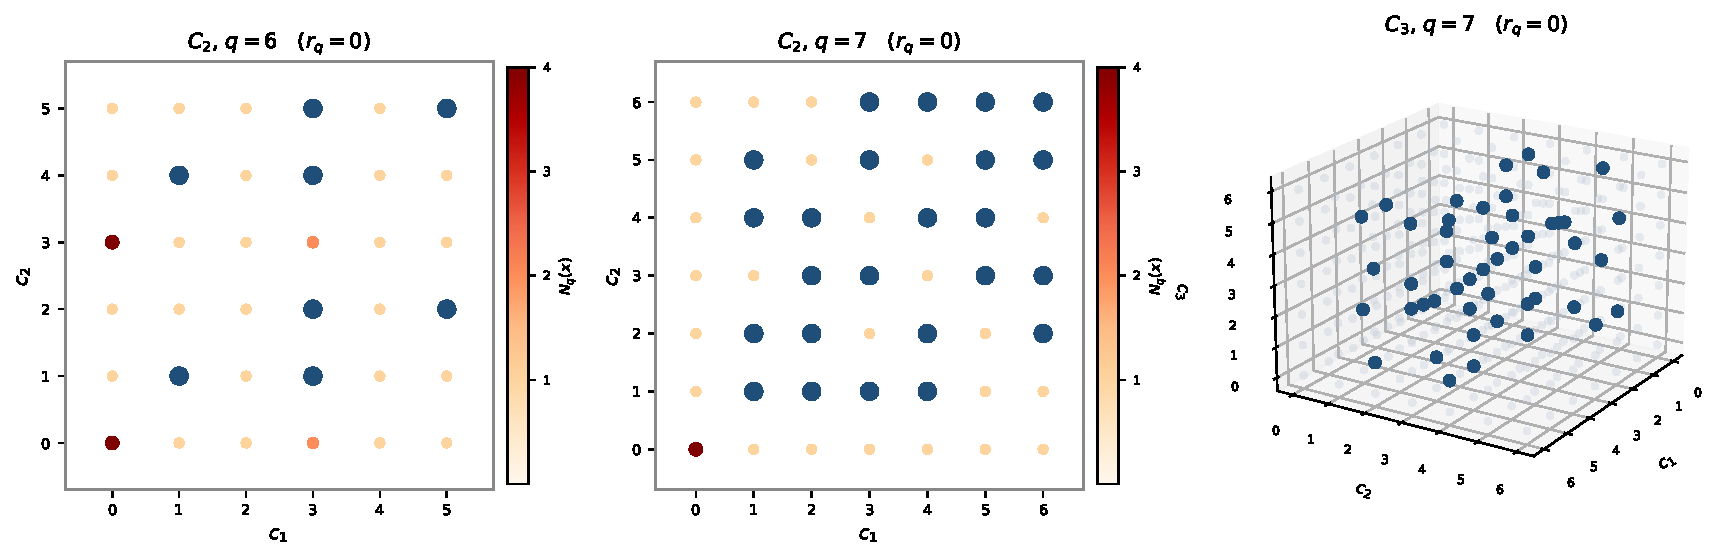
\includegraphics[width=\textwidth]{fig_walls.pdf}
\caption{The criterion is a point avoiding walls. Each dot is one weight modulo $q$, in the
coordinates $x=\sum_j c_j\omega_j$; blue means the character does not vanish there. The colour of the
others is $N_q(x)$, the number of walls the point does lie on --- the darker the point, the more
divisibilities $\lambda$ forces beyond what $\rho$ already forced. Left, $C_2$ at $q=6$, which is
$a_P$ itself: $\mathbf{8}$ survivors where $\prod_i(q-m_i)$ would give $15$. Middle, $C_2$ at $q=7$:
$\mathbf{24}$, and the product gives $24$. Right, the same picture one dimension up, $C_3$ at $q=7$:
$\mathbf{48}$, and the product gives $48$. The parity of $q$, and nothing else, separates the two
regimes. \ver{fig\_walls.py}}
\label{fig:walls}
\end{figure}


\noindent In type $C$ the count is closed for \emph{every} $q$, and in one statement. Write
\[
f=\begin{cases}1,&q\text{ odd},\\2,&q\text{ even},\end{cases}
\qquad a=\frac{q-f}{2},
\qquad m=uq+v \ \ (0\le v<q).
\]

\begin{theorem}[the count, every $q$, type $C$]\label{thm:cuenta}
\[
\boxed{\;
S_{C_m}(q)=
\begin{cases}
\dfrac{m!\;2^{\,2ua+v}\,\binom{a}{v}}
      {\bigl((2u+1)!\bigr)^{v}\,\bigl((2u)!\bigr)^{a-v}\,(u!)^{f}}, & v\le a,\\[6mm]
\dfrac{m!\;2^{\,a(2u+1)}\,\binom{a+f}{\,v-a\,}}
      {\bigl((2u+1)!\bigr)^{a}\,(u!)^{f}\,(u+1)^{\,v-a}}, & v>a.
\end{cases}\;}
\]
\end{theorem}

\noindent The proof is the marginal-cost argument of \S\ref{sec:cap} run backwards, and it never
used $q\mid 2m+2$: the cost of an extra row is $0,1,2,\dots$ in a non-fixed class and $1,3,5,\dots$
in a fixed one, so the minimum is attained by filling the cheapest places, and $\rho=(m,\dots,1)$
attains it --- its residues are $u$ full turns of $\ZZ/q$ followed by $1,\dots,v$. When $v\le a$
each fixed class carries $u$ rows, $v$ non-fixed classes carry $2u+1$ and the rest carry $2u$,
which the binomial $\binom{a}{v}$ chooses; each row of a non-fixed class has two possible residues,
which is the power of $2$. When $v>a$ one starts from $2u+1$ in every non-fixed class and $u$ in
every fixed one and places the remaining $b=v-a$ rows in distinct classes; adding a row multiplies
the weight by $1/(u+1)$ whether the class is fixed or not, so all $\binom{a+f}{b}$ choices weigh the
same. \emph{Checked against exhaustive enumeration on $40$ pairs $(m,q)$: no discrepancy.}
\ver{referee2.py}

\noindent \textbf{The two formulas of the earlier draft are the two ends of this one.} For $q>2m$
one has $u=0$ and $v=m\le a$, so $S_{C_m}(q)=m!\,2^m\binom{a}{m}$, which is
$\prod_i(q-(2i-1))$ for $q$ odd and $\prod_i(q-2i)$ for $q$ even --- exponents and degrees, as
above. For $q\mid 2m+2$ it returns the multinomial count over the capacities, and at $a_P$ itself
$S_{C_m}(2m+2)=2^m\,m!$. In the range that was open in between, it gives for instance
$S_{C_3}(5)=72$ and $S_{C_3}(6)=96$.

\begin{keybox}
\textbf{And a correction that matters more than the formula.} It is tempting to call $S_X(q)$ a
quasi-polynomial and go looking for its period. It is not one, globally. The literature on
characteristic quasi-polynomials counts the \emph{complement} of the modular arrangement --- the
points on no wall at all --- whereas $S_X(q)$ counts the stratum at the minimal level $r_q$, and
$r_q$ itself changes with $q$. The two agree only where $r_q=0$. Already in $C_2$ one has
$S_{C_2}(q)=(q-1)(q-3)$ for every large odd $q$, while $S_{C_2}(3)=8$ and not $0$; and no choice of
period repairs that, since any infinite progression of odd numbers containing $3$ forces the same
polynomial. The right statement is \emph{eventually} quasi-polynomial behaviour, with a distinct
singular regime --- which is exactly what Theorem~\ref{thm:cuenta} makes explicit.
\end{keybox}

\section{A test outside type $C$: $G_2$}\label{sec:g2}

The capacity rule is written in the coordinates of type $C$, so the honest question is what
survives outside them. I had meant to leave that open, and while writing this I tested it instead.
The reasoning was: a fixed class carries $\lfloor d/2\rfloor$ because the folding is an involution,
so in $G_2$, where $r=3$, it should carry $\lfloor d/3\rfloor$. I built the missing evaluator ---
Freudenthal multiplicities in $G_2$, checked against the Weyl dimension formula, and returning
$\{0,\pm1\}$ at $a_P$ itself, which is the control that says the element is the right one.

\begin{keybox}
\textbf{The prediction failed, and the right statement was next door.} At $k=1$ the naive criterion
transports exactly --- $\chi_\lambda(a_P)=0$ iff some positive root has $q\mid(\lambda+\rho,\alpha)$,
$49$ of $49$. Where the order drops --- $d>1$, which among $k=1,\dots,6$ means $k=2,3,4,6$; at
$k=5$ one has $d=1$ again and the naive rule still works --- it fails badly, the best of three
natural conditions giving $20$ of $49$.
But that is because at a power the denominator already carries $r_q$ forced zeros: asking whether
\emph{some} root divides is the wrong question. With \eqref{eq:crit} instead --- whether there are
\emph{more} divisibilities than $\rho$ has --- $G_2$ closes, and not as a measurement:
\eqref{eq:crit} is a statement about a root system, so it applies here exactly as it stands. The
values, meanwhile, leave $\{0,\pm1\}$ decisively: at $k=4$ they reach $343$.
\end{keybox}

\noindent In coordinates: with $\lambda=a\omega_1+b\omega_2$, $u=a+1$ and $v=3(b+1)$, the six values
$(\lambda+\rho,\alpha)$ are $u,\;v,\;u+v,\;2u+v,\;3u+v,\;3u+2v$. So $N_q(\ell)$ counts how many
of those six are divisible by $q$, and $r_q$ is the same count on $1,3,4,5,6,9$. Here $t=12$ and
$q=12/\gcd(k,12)$, and two values of $q$ collapse --- for \emph{every} dominant weight, not for the
ones I happened to run:

\begin{corollary}\label{cor:g2}
In $G_2$: at $q=3$ (that is $k=4,8$), $\chi_\lambda(a_P^k)=0$ if and only if $a\equiv2\ (3)$; and at
$q=2$ (that is $k=6$), $\chi_\lambda(a_P^k)=0$ if and only if $a\equiv b\equiv1\ (2)$.
\end{corollary}

\begin{proof}
At $q=3$, $v=3(b+1)\equiv0$, so the six values reduce to $u,0,u,2u,0,0$ and
$N_3=3+3\cdot[\,3\mid u\,]$, while $r_3=3$, the multiples of $3$ among $1,3,4,5,6,9$. Hence
$N_3=r_3$ exactly when $3\nmid u=a+1$. At $q=2$, $3u+v\equiv u+v$, $2u+v\equiv v$ and
$3u+2v\equiv u$, so the six reduce to $u,\,v,\,u+v$ each taken twice and
$N_2=2\,\#\{u,v,u+v \text{ even}\}$; among three numbers of which one is the sum of the other two,
either exactly one is even or all three are, so $N_2$ is $2=r_2$ unless $u$ and $v$ are both even,
when it is $6$. Hence $N_2=r_2$ fails exactly when $a$ and $b$ are both odd.
\end{proof}

\noindent \emph{Both congruences checked on all $\mathbf{40\,401}$ weights with $a,b\le200$, against
three altered congruences as decoys, each of which fails.} \ver{revision\_50\_G2\_corolario.py}
\emph{And the criterion itself against exact Freudenthal characters --- which is the control that
the criterion is the right one, not the proof --- $49$ of $49$ dominant weights for every
$k=1,\dots,6$, over $0\le a,b\le6$.} \ver{revision\_47\_G2.py}

\noindent What that says is not that $G_2$ has no theory, but that my prediction was not well posed.
``Fixed class'' presupposes the coordinates $e_i$ and the involution on residues that type $C$ has;
$G_2$ has neither, so $\lfloor d/r\rfloor$ was a guess wearing the clothes of a consequence. The
capacity picture looks like a fact about the \emph{coordinates} of type $C$, not about the ratio of
root lengths. What plays the part of a class in general is not another set of buckets but the map
\[
c_q(\lambda):Q\longrightarrow\ZZ/q,\qquad \alpha\longmapsto(\lambda+\rho,\alpha)\bmod q,
\]
taken up to $W$ --- an element of $\operatorname{Hom}(Q,\ZZ/q)/W$. In $C_m$, written on
$e_i-e_j,\ e_i+e_j,\ 2e_i$, that datum decomposes into exactly the folded buckets $x\sim-x$. In
$G_2$ it is the point $(u,v)$ and its incidence with the six root walls $u=0$, $v=0$, $u+v=0$,
$2u+v=0$, $3u+v=0$, $3u+2v=0$ modulo $q$; and $N_q(\ell)$ counts how many of them contain it. So
the general notion is a point of rank two and an arrangement, not a one-dimensional bucket.
\ver{G2\_caracteres.py}

I also tried to derive the $G_2$ criterion and got it wrong, in a way worth recording: I argued that
if a reflection leaves the exponent fixed modulo $q$ then its two terms cancel. They do --- but two
terms out of $|W|$. The true statement is that the Weyl numerator vanishes whenever the stabiliser
of the element contains a reflection, which is to say \emph{whenever the element is not regular},
which is every case with $d>1$. So the numerator says nothing there, and one is back at the limit
--- the same limit of \S\ref{sec:cierre}.





\begin{keybox}
\textbf{And at $q=3$ the value itself closes, sign included.} With $\lambda=a\omega_1+b\omega_2$,
$u=a+1$ and $v=3(b+1)$, the exponents divisible by $3$ on a surviving weight are $v$, $3u+v$ and
$3u+2v$, against $3,6,9$ for $\rho$; the other three factors have equal modulus on the two sides,
and the floors of \S\ref{sec:valor} give the sign. Hence, for $k=4$ and $k=8$,
\[
\chi_{a\omega_1+b\omega_2}(a_P^{\,k})=
\begin{cases}
\ \ \dfrac{(b+1)(a+b+2)(a+2b+3)}{6}, & a\equiv0 \ (3),\\[3mm]
-\dfrac{(b+1)(a+b+2)(a+2b+3)}{6}, & a\equiv1 \ (3),\\[3mm]
\ \ 0, & a\equiv2 \ (3).
\end{cases}
\]
At $a=b=6$ this gives $7\cdot14\cdot21/6=343$, which is the value the measurement above reports ---
now for the whole family rather than for the sample.
\end{keybox}


\section{One piece of \cite{NPP25} with a single weight changed}\label{sec:types}

\noindent Everything above counts roots: the criterion, the capacities, the value, the survivors.
Which roots, exactly --- and is the set they form one the literature has already classified? It
is, with a single weight changed.

The $R(m)$ of \cite{NPP25} selects roots by height, $\langle\beta,\rhoh\rangle$. Kostant's normalisation makes
$\langle\alpha,x_P\rangle$ proportional to $(\alpha,\alpha)$, so for $a_P$ the statistic gives weight
$1$ to short simple roots and $r$ to long ones. Call it the $P$-height. Then
\[
\hgt_P(\alpha) \;=\; \tfrac{(\alpha,\alpha)}{2}\,\hgt(\alpha^\vee) \;=\; (\rho,\alpha),
\]
the second equality being immediate from $\alpha^\vee=2\alpha/(\alpha,\alpha)$ and
$\langle\rho,\alpha_i^\vee\rangle=1$. So the $P$-height \emph{is} the root statistic of
\eqref{eq:ps}, and the set $R_P(q)$ of \S\ref{sec:crit} --- whose size gave $r_q$ --- is the set of
roots of $P$-height divisible by $q$. That is the only reason this section belongs in this note.
\emph{Both readings checked to agree on every positive root of $B_3,B_4,C_3,C_4,C_5,F_4,G_2$ and
every $q\le24$, with the plain coheight as a decoy, which differs.} \ver{revision\_52\_bisagra.py}
And:

\begin{observation}\label{obs:types}
Read through coroots, $R_P(q)$ always contains $R(q)$ computed in the dual group; the extra part is
exactly the long roots $\alpha$ of $G$ with $q \mid r\,\hgt(\alpha^\vee)$ but $q\nmid\hgt(\alpha^\vee)$;
and the two coincide whenever $\gcd(q,r)=1$.
\end{observation}

\begin{proof}
Under $\alpha\leftrightarrow\alpha^\vee$ the identity above reads $\hgt_P(\alpha)=\hgt(\alpha^\vee)$
for $\alpha$ short and $\hgt_P(\alpha)=r\,\hgt(\alpha^\vee)$ for $\alpha$ long. So $q\mid
\hgt(\alpha^\vee)$ implies $q\mid\hgt_P(\alpha)$ in both cases, which is the containment; the
converse fails only for a long $\alpha$ with $q\mid r\,\hgt(\alpha^\vee)$ and
$q\nmid\hgt(\alpha^\vee)$, which is the stated extra part; and if $\gcd(q,r)=1$ then
$q\mid r\,\hgt(\alpha^\vee)$ forces $q\mid\hgt(\alpha^\vee)$, so there is no extra part.
\end{proof}

\noindent That is three lines, so the measurement below is a control and not the evidence:
Figure~\ref{fig:types} draws where the two selections part company.
$\mathbf{186}$ pairs (type, $q$) --- $B_n$ and $C_n$ up to $n=5$, $F_4$ and $G_2$, each
with $2\le q\le 2h+1$ --- all three clauses without exception. \ver{R\_P\_todos\_los\_tipos.py}

\noindent \textbf{What that does not give.} When $\gcd(q,r)=1$ the two selections coincide and the
classification of \cite{Polo25} --- which is a classification of the subsystems cut out by
divisibility of the \emph{ordinary} height --- transfers to the $a_P$ side directly. When
$\gcd(q,r)>1$ it does not: the extra long roots can change the type of the subsystem, and in $G_2$
at $q=3$ they do. There $R_P(3)$ contains the three positive long roots and is of type $A_2$, while
the selection by coheight divisible by $3$, before the extra roots are added, has a single positive
root. The observation stands; the classificatory consequence needs an argument this note does not
give.

\begin{figure}[tbp]
\centering
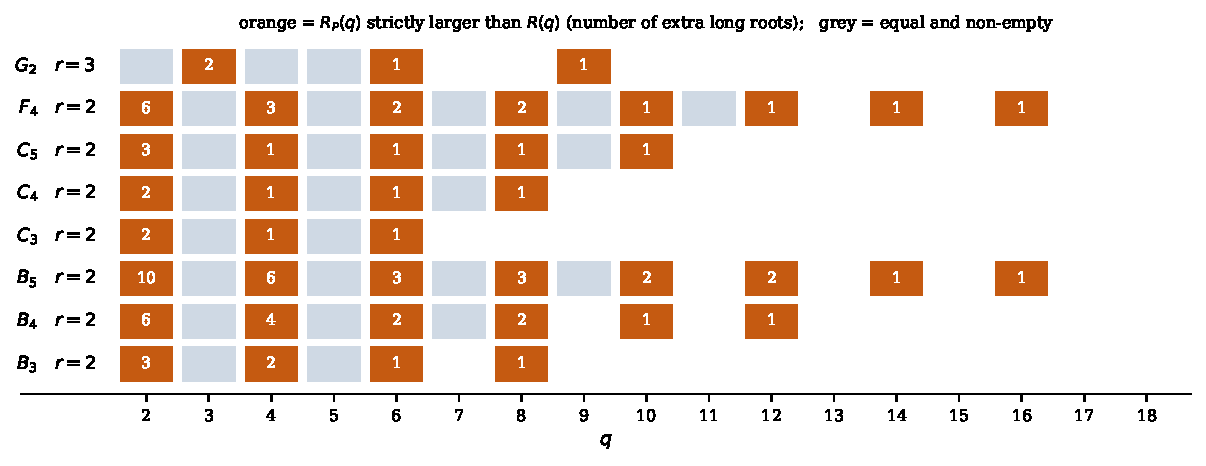
\includegraphics[width=\textwidth]{fig_types.pdf}
\caption{$B$, $C$ and $F_4$ part company only at even $q$; $G_2$ only at $q=3,6,9$, the multiples of
its $r=3$. The number in each orange cell is how many extra long roots $R_P(q)$ carries.}
\label{fig:types}
\end{figure}

\noindent The converse of the last clause is false for a dull reason --- for large $q$ both sets are
empty. I mention it because my first version was an ``if and only if'' with $32$ counterexamples,
$26$ of them exactly that and the other $6$ a transposed Cartan matrix of $G_2$ on my side.


\section{What this is not}\label{sec:open}

\begin{itemize}\itemsep2pt
\item \textbf{The engine is not mine.} Equation~\eqref{eq:ps} is the classical principal
specialisation; all I did was read it on the line of $\rho$, which is where Kostant's second element
lives. What is added here is the zero-count \eqref{eq:crit}, the classification of the denominators at
which the values are whole (Theorem~\ref{thm:clasif}), and the combinatorics that turns the
count into capacities.
\item \textbf{What is open is outside type $C$.} Corollary~\ref{conj:cap} settles the vanishing in
type $C$ and Theorem~\ref{thm:crit} settles it in any type. Inside type $C$ the value is complete:
Theorem~\ref{thm:valgen} gives the absolute value for every $k$, the Lemma~\ref{lem:unit} it is
conditional on is Proposition~\ref{prop:Ms} at $d=2$ and Proposition~\ref{prop:res} at every $d$,
and Theorem~\ref{thm:signo} gives the sign. What is \emph{not} proved is Lemma~\ref{lem:unit}
outside type $C$, where \eqref{eq:res} has no analogue yet. And the sign, though determined, does
not simplify: \S\ref{sec:cierre} records where a shorter form was looked for and is not.
\item \textbf{The criterion is type-independent; the capacities are type $C$.}
Theorem~\ref{thm:crit} is a statement about a root system: in $C_m$ it becomes
Corollary~\ref{conj:cap}, in $G_2$ the six-wall criterion of \S\ref{sec:g2}. Observation~\ref{obs:types}
is likewise about root systems, not characters. Characters themselves I can compute in $C_m$ and in
$G_2$, but not in type $B$, where I would need the $\SO(2m+1)$ character.
\item \textbf{No transport of \cite{Prasad16} is claimed.} The proof of Theorem~\ref{thm:crit} is
self-contained and uses no result of \cite{Prasad16}; whether the argument of that paper also reaches
this criterion is a question this note does not address.
\item Of \cite{Polo25} I have read the introduction, \S2 and enough of \S3.3 to confirm the selection
is by height throughout; the case-by-case proofs I have not read.
\end{itemize}


\section{What this leaves}\label{sec:preguntas}

In the family $q\mid t$ the value, its sign and the count are settled above, and the one step
that was a measurement --- the triviality of the non-vanishing factor --- is now
Proposition~\ref{prop:res}. But Theorem~\ref{thm:clasif} has widened the ground under all of
that: there are three further families where every character is a whole number and where this
note evaluates nothing. What follows are the questions that remain, the first of which did not
exist before \S\ref{sec:clasif}, and two of the others are sharper than they look because the
obvious answer has a counterexample.

\begin{enumerate}\itemsep5pt

\item \textbf{What is the value in the other three families?}
Theorem~\ref{thm:clasif} lists four families of denominators at which every character is an
integer, and \S\ref{sec:valor} evaluates one of them. In the other three the construction of
\S\ref{sec:dims} still runs --- the keybox there reports $Z_q(\ell)/Z_q(\rho)=\kappa_q\,D$ over
every $q$ measured --- but the character is not $\pm\kappa_q D$: a further factor appears, and
the smallest case of it is already in \S\ref{sec:clasif}, where $\Sp(4)$ at $q=4$ has
$Z_4(\ell)/Z_4(\rho)=1$ and $\chi_{(1,0)}=-2$. \emph{What that factor is is no longer open.}
Proposition~\ref{prop:resid} identifies the difference of the two residue histograms as another
root system's, of rank at most $\lfloor q/2\rfloor$, and the box after it reads the factor off as
the character of that system at the same denominator --- over $\mathbf{1\,814}$ surviving weights
and at every $q$, not only at the classified ones. On the classified points that character takes
the values $1,2,3,4$ and $6$, and never anything else, over $\mathbf{828}$ surviving weights with
$m\le5$ and $q\le12$. \emph{What is left is the step from the identity to the value:} the passage
from the histogram to the absolute value and to the sign, and the cancellation of the constants of
\S\ref{sec:dims} at every $q$ rather than at $q\mid t$ --- that cancellation is measured over
$\mathbf{2\,186}$ surviving weights and proved only for $q\mid t$. \emph{What it would buy:} the
value on the whole classified set rather than on a quarter of it, and on the unclassified points
as well. \ver{teorema\_II.py, residual\_histogramas.py}

\item \textbf{Which group has the $D_c$ as its representations?}
Theorem~\ref{thm:dims} writes the modulus as a product of dimensions for $GL_n$, $Sp_{2n}$ and
$SO_{2n+1}$, and for odd $d$ the block profile is the same for every surviving $\lambda$
(\S\ref{sec:dims}). The natural guess --- a centraliser --- is \textbf{false on both sides}. Take
$m=6$, $k=7$, so $d=7$ and $q=2$: the two fixed classes carry three rows each, the factorisation
group is $Sp_6\times SO_7$, of type $C_3\times B_3$; but $a_P^{\,7}$ has eigenvalues $1$ and $-1$
with multiplicity six each, so $Z_{\Sp(12)}(a_P^{\,7})=Sp_6\times Sp_6$, of type $C_3\times C_3$.
Nor can $C_3\times B_3$ occur in the dual $SO(13)$: an eigenspace decomposition there produces
general linear and orthogonal factors, never a simple $C_3$. \emph{One construction that does mix them, and is worth testing:} inside the superalgebra
$\mathfrak{osp}(1|2m)$, whose even part is $\mathfrak{sp}_{2m}$ and whose odd part is the natural
representation, take the fixed subalgebra of $\mathrm{Ad}(-s_{\ell,q})$ rather than of
$\mathrm{Ad}(s_{\ell,q})$. On the even part the sign is invisible and one gets the usual
centraliser; on the odd part being fixed means lying in the $(-1)$-eigenspace, so only the class
$q/2$ keeps an odd part, and it assembles with its symplectic block into
$\mathfrak{osp}(1|2n_{q/2})$. \emph{Checked by dimensions on $\mathbf{1\,386}$ cases, $m\le7$ and
$q\le12$: the fixed subalgebra has exactly the dimensions of
$\bigoplus_c\mathfrak{gl}_{n_c}\oplus\mathfrak{sp}_{2n_0}\oplus\mathfrak{osp}(1|2n_{q/2})$, with no
exception; at $m=6$, $q=2$ it is $\mathfrak{sp}_6\oplus\mathfrak{osp}(1|6)$, of dimensions $42$ and
$6$.} \ver{osp.py} That the odd orthogonal dimensions come back is then the classical
correspondence between $\mathfrak{osp}(1|2n)$ and the non-spin representations of
$\mathfrak{so}_{2n+1}$. \emph{But this is not yet an answer:} nothing here builds the module out
of $V_\lambda$, and the subalgebra depends on the shifted datum $\ell$, not on the element alone.
\emph{Test:} find the construction on $V_\lambda$ whose fixed subalgebra this is. \emph{What it would buy:} Theorem~\ref{thm:dims} as a branching rule
instead of an identity of numbers.
\emph{And what is known for the neighbouring object:} for the full alphabet --- the fingerprint
of \S\ref{sec:dims} --- Lecouvey proves that in
the stable range $n>\max(\ell\,l(\lambda),l(\lambda'))$ the plethysm coefficients \emph{are}
branching coefficients for a Levi, the symplectic ones through $V^{\mathfrak{so}_{2n+1}}(\lambda')$
\cite[Thm.~4.5.1]{Lec07b}, while at even $\ell$ outside that range they are \emph{not}, and their
signs alternate \cite[Prop.~3.2.5]{Lec07a}. Neither settles the question here --- the object below
is one value, on a shorter alphabet --- but they say where the obstruction sits, and it is the
type-$B$ lattice obstruction of \S\ref{sec:dims} again.

\item \textbf{What do the two deleted letters do to the quotient?}
For the \emph{undeleted} alphabet the answer is \cite{Lec07a} and \cite{AK22}: the factors are
indexed by the components of $\mathrm{quo}_t(\lambda)$, and the folding into classes is already
Lecouvey's, fifteen years earlier. Here the $\nu^{(c)}$ of \S\ref{sec:dims} are built by hand,
and the natural guess is that they are the components of a $q$-quotient for the deleted alphabet.
The analogy has to be stated carefully: in type $A$ the classical core criterion is about a
specialisation at a \emph{full} multiset of $q$-th roots of unity and is false for an arbitrary
principal specialisation --- $s_{(1)}(1,-1,1)=1$ although $(1)$ has non-empty $2$-core.
\emph{Test:} compare $\nu^{(c)}$ with $\mathrm{quo}_q$ of the beta-set of $\lambda$ where both are
defined, and see what the two deletions move. \emph{What it would buy:} \S\ref{sec:dims} as a
corollary of \cite{AK22} rather than as a parallel identity.

\item \textbf{Outside type $C$, the open half is the modulus, not the sign.}
The sine derivation of Theorem~\ref{thm:signo} does not use the type: with the normalisation of
\S\ref{sec:norm} it gives the sign wherever the criterion applies. What was thought to be type $C$
is Proposition~\ref{prop:res} --- and \eqref{eq:adj} says its first half is not: it holds in every
type. What does \emph{not} generalise is the shape: $\mathrm{Sym}^2$ and $\Lambda^2$ of the
natural representation cover the classical types and say nothing about the exceptional ones,
where the only statement is \eqref{eq:adj} itself. Its second half holds
wherever $\ell$ lies in the orbit $\widehat W_q^{+}\!\cdot\rho$, again in every type. \emph{So what
is actually open is the free place:} the surviving weights outside that orbit, which occur exactly
for $d$ even with $q\ge3$. \emph{Test:} settle those in $B_m$ and $F_4$, where the ratio of root
lengths is again $2$ but the coordinates differ. \emph{The measurement says it is worth trying:}
$\mathscr{R}_\ell=\mathscr{R}_\rho$ was checked on all $\mathbf{1\,463}$ surviving weights of
$B_2,B_3,B_4$ and all $\mathbf{861}$ of $G_2$ over the five $q\mid12$ --- no exception, in types
where this note proves nothing. \ver{lema\_generico.py} \emph{And a warning that any such extension has to respect:} the closed form is
\textbf{not} valid at an arbitrary point of the $\rho$-line, even in type $C$. In $\Sp(4)$ with
$\lambda=(1,0)$ and $q=7$ no exponent is divisible by $7$, so $Z_7(\ell)/Z_7(\rho)=1$, while
$\chi_{(1,0)}(g_{1/7})=2\cos\frac{2\pi}{7}+2\cos\frac{4\pi}{7}=0.8019\ldots$ The criterion holds along the whole line; the \emph{value} formula is a statement about the
classified points of Theorem~\ref{thm:clasif}, and $q=7$ with $m=2$ is not one of them.

\item \textbf{What is the count outside type $C$?}
Theorem~\ref{thm:cuenta} closes $S_{C_m}(q)$ for every $q$, and \S\ref{sec:cuenta} records that in
the regular regime the answer reads by exponents at odd $q$ and by degrees at even $q$. That
alternation is exact in $A$ and $C$ and \emph{breaks in $B_3$}, whose weight lattice carries the
spin weight. \emph{Test:} redo the marginal-cost count in $B_m$ and $D_m$ with $P$ rather than
$\ZZ^m$, and see whether the lattice index enters as a factor or changes the shape.
\emph{What it would buy:} one counting theorem for the classical types instead of one for $C$, and
the beginning of an answer for the exceptional ones.

\item \textbf{The $\rho$-line does not contain $a_Q$: what family contains both?}
It is tempting to read \S\ref{sec:crit} as putting Kostant's two elements on one line, and that is
false. In $\Sp(4)$ the lift of $a_Q$ used in \S\ref{sec:controles} has spectrum
$\{\zeta_8,\zeta_8^3,\zeta_8^5,\zeta_8^7\}$, while a point of the $\rho$-line has spectrum
$\{z,z^{-1},z^2,z^{-2}\}$; if $z$ were one of those eigenvalues it would have order $8$, and then
$z^2$ would have order $4$ and not lie in the spectrum of $a_Q$. No $z$ works. \emph{Test:} take the
two-parameter family $\exp(2\pi i(\theta\rho^\sharp+\theta'\rho^{\vee\sharp}))$ and ask on which of
its points the argument of \S\ref{sec:crit} still closes. \emph{What it would buy:} the unification
that \S\ref{sec:map} draws as two lines meeting at a box, stated as mathematics rather than as a
picture.

\end{enumerate}

\appendix
\section{What was tried on the way, and did not work}\label{sec:cierre}

\noindent \emph{What follows is a record, not a result.} Corollary~\ref{conj:cap} says that at
$z=\xi_q$ the two sides of \eqref{eq:ps} vanish to the same order, so the character is a limit
--- and a limit is a computation, not a programme. \S\ref{sec:modulo} does that computation.
What is kept here is the road taken before it was found, because a reader deciding how much to
trust the result should be able to see which of the obvious routes were tried and where each
of them stopped. So:

\begin{keybox}
\textbf{Problem.} At $z=\xi_q$ the numerator and denominator of \eqref{eq:ps} vanish to the same
order --- that is exactly \eqref{eq:crit}, which is Corollary~\ref{conj:cap} --- so the character is
the limit
\[
\chi_\lambda(a_P^k)\;=\;\xi_q^{-(\lambda,\rho)}\lim_{z\to\xi_q}\ \prod_{\alpha>0}
\frac{1-z^{(\lambda+\rho,\alpha)}}{1-z^{(\rho,\alpha)}} .
\]
\textbf{That limit is now evaluated, and what it leaves is a lemma and a sign.} Factoring out the
$r_q$ vanishing factors on each side gives the ratio of the products of their exponents --- there is
no canonical root-by-root pairing, and none is needed. That is Theorem~\ref{thm:valgen}, and it
holds at every $d$ provided the surviving factors contribute nothing to the modulus, which is
Lemma~\ref{lem:unit}: proved at $d=2$ by Proposition~\ref{prop:Ms} and, in type $C$, at every $d$ by
Proposition~\ref{prop:res}. \textbf{So what is left of this route is outside type $C$}, where
\eqref{eq:res} has no analogue yet --- and there too the lemma is finite arithmetic, two explicit
products of $1-\xi_q^{\,r}$ with the same modulus, with no representation theory in sight.
\end{keybox}

\smallskip
\noindent\textbf{Two things the sign is not.} Theorem~\ref{thm:signo} gives the sign as a sum of
floors, and \S\ref{sec:valor} shows that the tidier candidate does not survive checking. What
follows is the rest of that search, worth recording because it says how fine an invariant the sign
is. At $k=2$ the alphabet gives
$H(z)=(1-z)^2/(1-z^q)^2$, so the character is an integer determinant and its sign is a hard datum,
with no numerical judgement in it. Over $\mathbf{4\,301}$ surviving weights in $\Sp(2m)$ for
$m=2,\dots,9$, Theorem~\ref{conj:val} holds without a single discrepancy --- which also extends its
verification to $m=7,8,9$. On that sample:

\begin{itemize}\itemsep2pt
\item the sign is \textbf{not a function of the occupancy pattern}. Of the $32$ patterns of ``which
classes hold $0$, $1$ or $2$ rows'' that occur, \emph{none} carries a constant sign. The smallest
witness is in $\Sp(4)$ at $k=2$: $\lambda=(1,0)$ and $\lambda=(1,1)$ occupy the same classes and
have the same modulus $2$, and their characters are $-2$ and $+2$. The sign reads the numbers,
not the shape.
\item and it is \textbf{not a $\mathrm{GF}(2)$-linear combination} of fifteen natural parities: the
number of classes taking the $+$ branch of $\mp$ and the number taking the $-$, the parity of the
quotients $\lfloor\ell_i/q\rfloor$, of the folded rows, of $|\lambda|$, of $(\lambda,\rho)$, of the
inversions of the class word, the index of the free class, and others. The linear system over the
$2\,582$ weights with $m\le6$ is \emph{inconsistent} --- no subset of them works, so none had to be
validated on the $1\,719$ weights of $m=7,8,9$ that were held back for that. A column of random
parities rode through the fit as a decoy.
\end{itemize}

\noindent That is a negative result, and it is what makes the second item below worth someone's time
rather than an afternoon's: the sign is a finer invariant than the natural candidates, and the
place a shorter form is most likely hiding is the same one the modulus came from --- the Weyl
element that arranges the residues, whose length is not a function of the classes alone.
\ver{sign\_k2.py}

\noindent The other way in is the finite difference of \S\ref{sec:alph} --- the question left
hanging there. It has an answer, and I had it backwards for two days, so I record both. I thought
the obstruction was that the shift acts on $b_i+j$ and $b_i-j$ with opposite signs and therefore does
not factor out. It does factor out. The shift moves the \emph{index} of $h$, and $h_{b_i\pm
j}\mapsto h_{(b_i-1)\pm j}$ is a shift of $b_i$ in \emph{both} summands; the sign of $j$ never
enters. So, by multilinearity in rows, for any polynomial $P$,
\[
D_{P(S)h}(\mathbf b)=\Bigl(\prod_{i=1}^{m}P(T_i)\Bigr)D_h(\mathbf b),
\qquad (T_iF)(\dots,b_i,\dots)=F(\dots,b_i-1,\dots),
\]
and in particular $D_A=\prod_i(1-T_i)^2 D'$ for $d$ even and $\prod_i(1-T_i^2)D'$ for $d$ odd.
\emph{Checked numerically to $10^{-14}$, with a decoy that fails.}
\ver{revision\_47\_verificacion.py}

So the branching is not the obstacle I made it out to be, and the second difference does
pass through the determinant. What remains on that route is the cancellation among determinants with
shifted beta-numbers --- and none of it is needed any more inside type $C$, where \eqref{eq:crit}
settles the vanishing and Proposition~\ref{prop:res} the value. Outside it I would still start from
the limit in the box above, because it carries the exponents explicitly.

One place worth looking, which I only found late: Kumari's second paper \cite{Kum24}
treats $\Sp_{2tn+2}$ --- the big alphabet \emph{plus} one extra pair. What this note needs is the big
alphabet \emph{minus} one pair. That is the adjacent case, done with Weyl character formulas and
beta-sets of $t$-cores, and if the machinery there runs backwards it may be the whole answer.

And that is where it stops. What I would most like to know, in order:
\begin{itemize}\itemsep2pt
\item \textbf{Lemma~\ref{lem:unit} outside type $C$.} Inside it, statement (B) of
\S\ref{sec:modulo} proves the lemma and with it all of Theorem~\ref{thm:valgen}, and (B) is a
congruence between two multisets of residues with no characters anywhere in it. What it rests on is
\eqref{eq:res}, which is written in the coordinates of type $C$; the same congruence elsewhere is
the whole of what the value still needs;
\item a \textbf{shorter form of the sign} than the sum of floors --- and the two negative results
above say it is neither a function of the occupancy pattern nor a parity of the natural statistics;
\item whether the row lemma plus the cancellation among shifted determinants gets there by the
other road, and whether Kumari's $\Sp_{2tn+2}$ \cite{Kum24} run backwards is that cancellation.
\end{itemize}

\section{The controls, in the order they were run}\label{sec:controles}

None of what follows is needed for a proof. It is kept because the statements above were measured
before they were derived, and a reader deciding how much to trust them should be able to see what
was actually run.


\subsection*{First, Theorem~2 of \cite{Prasad16b} --- recomputed, not cited}

At $t=1$ --- again the torus element of that paper, not the $2m+2$ of this one --- the alphabet in
its Theorem~2 is
$\mu_n$ with multiplicity $m$, so
$H(z)=\prod_{\omega^n=1}(1-\omega z)^{-m}=(1-z^n)^{-m}$, the $h_k$ are integers and the determinant
is exact. I implemented the statement from scratch and ran it.

\begin{center}
\small
\rowcolors{2}{white}{filaclara}
\begin{tabular}{ccrccc}
\toprule
\rowcolor{cabecera}$m$ & $n$ & weights & criterion & value & decoys (one block fewer / more)\\
\midrule
1&3& 84 & $84/84$ & $84/84$ & $27$ / $27$\\
2&2& 210 & $210/210$ & $210/210$ & $40$ / $40$\\
2&3& 462 & $462/462$ & $462/462$ & $72$ / $54$\\
3&2& 462 & $462/462$ & $462/462$ & $60$ / $40$\\
2&4& 495 & $495/495$ & $495/495$ & $54$ / $54$\\
3&3& 220 & $220/220$ & $220/220$ & $32$ / $32$\\
4&2& 495 & $495/495$ & $495/495$ & $45$ / $45$\\
\midrule
\multicolumn{2}{c}{total} & $\mathbf{2428}$ & $100\%$ & $100\%$ & \\
\bottomrule
\end{tabular}
\end{center}

\noindent The last column is the control: a formula using one block fewer, or one more, agrees
between $8.7\%$ and $32.1\%$ of the time. \ver{prasad2016\_vs\_nuestro.py}


\subsection*{Second, the other element}

With $\ell=\lambda+\rho$, $d=\gcd(k,t)$ and $q=t/d$:

\noindent I measured a rule about capacities first --- the $31$ pairs $(m,k)$ with $m=2\ldots7$,
$k=1\ldots6$ and $q\ge3$, over $\lambda_1\le8$ (or $\le6$ for $m\ge5$): $\mathbf{21\,630}$ dominant
weights, no exception \ver{aP\_potencias.py} --- and then, once Proposition~\ref{prop:alph} told me
the element sits on the $\rho$-line, it turned out to be the shadow in type $C$ of something that
does not mention type $C$ at all.

\smallskip

\subsection*{Third, the control: the same test on Kostant's other element}

A rule that fits could still be a rule about ladders rather than about $a_P$. So I ran the same test
on $a_Q$ inside the same group. In $\Sp(2m)$ the Coxeter element is the odd ladder
$(1,3,\dots,2m-1)$ at order $4m$ --- $\rhoh$ is half-integral, so the lift has order $2h$ --- and I
checked that it pairs to $1$ on every simple root, which the even ladder does not.

Then, for each $(m,k)$, I asked which pairs (capacity on a non-fixed class, capacity on a fixed one)
out of all pairs in $\{0,\dots,4\}^2$ reproduce the vanishing exactly.

\begin{keybox}
For $a_P$ the answer is always $(d,\lfloor d/2\rfloor)$ and nothing else. \textbf{For $a_Q$ there is
usually no answer at all}: in $14$ of the $16$ cases run, \emph{no} pair of capacities reproduces the
vanishing. So the rule is not a fact about ladders. It is a fact about $a_P$, and
Proposition~\ref{prop:alph} says why: the alphabet of $a_Q^{\,k}$ is supported on the \emph{odd}
residues, and is not $d\cdot\mu_q$ minus two points at all.
\end{keybox}

\noindent That is the control I would have most wanted someone to run against me, so I ran it before
sending this. \ver{aQ\_potencias.py}


\section*{Attribution}\label{tab:attrib}

{\small
\rowcolors{2}{white}{filaclara}
\begin{longtable}{@{}p{0.40\textwidth}p{0.55\textwidth}@{}}
\toprule
\rowcolor{cabecera}the alphabet, as a multiset of $\mu_q$ & who has it\\
\midrule
\endfirsthead
\toprule
\rowcolor{cabecera}the alphabet, continued & \\
\midrule
\endhead
$c\cdot\mu_q$ \emph{exactly} --- the full alphabet
 & Littlewood \cite{Li40}; Prasad \cite{Prasad16b}, Thm.~2, on $\GL$;
   Ayyer--Kumari \cite{AK22} on the classical groups; Albion \cite{Alb23} on the universal
   characters; and Lecouvey \cite{Lec07a,Lec07b}, independently, through plethysm --- the joint
   attribution is Albion's own \cite{Alb25}\\
$c\cdot\mu_q$ \emph{plus} a partial run of $m$ letters & Kumari \cite{Kum24}, Thm.~2.2\\
\textbf{the three types on the folded classes --- $C$ on the class $0$, $A$ on the folded pairs, $B$
on the class $q/2$ --- and that at even $\ell$ they are not branching coefficients}
 & \textbf{Lecouvey \cite{Lec07a}}, \S3.2.2, Thm.~3.2.3 and Prop.~3.2.5, on the \emph{full}
   alphabet; stably, and through $V^{\mathfrak{so}_{2n+1}}(\lambda')$, \cite{Lec07b}, Thm.~4.5.1\\
$c\cdot\mu_q$ \emph{plus} one letter $1$ & Kumari \cite{Kum24}, Thm.~2.8\\
supported on the \emph{odd} residues --- which is the alphabet of $a_Q$, not of $a_P$
 & Ayyer--Kumari \cite{AK25}, \S3\\
any alphabet at $q=2$ --- the elements of order $2$ & Karmakar \cite{Kar24}, Thm.~5.1\\
\midrule
\rowcolor{marca}$c\cdot\mu_q-\{1\}-\{-1\}$ (Prop.~\ref{prop:alph}, $d$ odd) & this note\\
\rowcolor{marca}$c\cdot\mu_q-2\cdot\{1\}$ (Prop.~\ref{prop:alph}, $d$ even) & this note\\
\midrule
$c\cdot\mu_q-\{1\}$ --- one letter, at the fixed point
 & \emph{no source found in the literature checked here}\\
\bottomrule
\end{longtable}}

\vspace{4pt}
\noindent That is the axis, because the alphabet decides both what is true and what is whose.
Every alphabet in the upper block is a whole multiple of $\mu_q$, or that with a short run
added; the two rows of this note are that multiple \emph{short of} at most two letters, and
those letters are the fixed points of $w\mapsto w^{-1}$. The row with no source is a third of
the same kind, which the argument of \S\ref{sec:modulo} covers and which is not stated below.
\emph{This is a description of the families listed, not a classification of the $\rho$-line:
there are denominators outside all of them where the non-vanishing factor still cancels ---
$\Sp(14)$ at $q=6$ is one, and its alphabet is not of this shape at all.}
\ver{alfabeto\_clasif2.py}

\vspace{6pt}
{\small
\rowcolors{2}{white}{filaclara}
\begin{longtable}{@{}p{0.52\textwidth}p{0.43\textwidth}@{}}
\toprule
\rowcolor{cabecera}the rest of what this note stands on & \\
\midrule
\endfirsthead
\toprule
\rowcolor{cabecera}attribution table, continued & \\
\midrule
\endhead
$\{0,\pm1\}$ at $a_Q$ and at $a_P$; the two elements & Kostant \cite{Kostant76}\\
twisted $=$ folded, and $A_{2m}\to C_m$ & Kumar--Lusztig--Prasad \cite{KLP09}\\
the Weyl-group shadow, $\Theta(w_0)=\pm\dim$ & L\"ubeck--Prasad \cite{LP20}\\
$R(m)$, $d_m$, and its classification & NPP \cite{NPP25}, Polo \cite{Polo25}\\
the type-$C$ rule as a Macdonald identity & P\'etr\'eolle \cite{Petreolle15}, Wahiche \cite{Wahiche23}\\
the type-$A$ rule with cores & Adin--Frumkin \cite{AF02}\\
\midrule
the principal specialisation \eqref{eq:ps} & classical\\
\textbf{the criterion \emph{and} the sign at $a_P$ itself, in every type; its type-$C$ form; and the
sign read off the ordered residues} & \textbf{Cellini--M\"oseneder Frajria--Papi \cite{CMP06}},
Cor.~3.2, Prop.~3.5 and Rem.~3.2\\
the coroot form of the criterion, for every integer & NPP \cite{NPP25}, Cor.~3.7\\
\midrule
\rowcolor{white}\multicolumn{2}{l}{\emph{and what is done here, beyond the two alphabet rows above:}}\\
\textbf{which denominators of the $\rho$-line give integer values} (Thm.~\ref{thm:clasif}) & \\
the same count on the whole $\rho$-line, at the powers (Thm.~\ref{thm:crit}) & \\
the combinatorics that turns it into capacities (Cor.~\ref{conj:cap}) & \\
the one unit of slack, and where it comes from (Prop.~\ref{prop:slack}) & \\
the absolute value at $k=2$ (Thm.~\ref{conj:val}) & \\
the absolute value at any $k$ (Thm.~\ref{thm:valgen}), modulo Lem.~\ref{lem:unit} & \\
the residue lemma \eqref{eq:res}, and \eqref{eq:adj} behind it (Prop.~\ref{prop:res}) & \\
the exact value with its sign, \emph{every} power, type $C$ (Thm.~\ref{thm:signo}) & \\
its modulus factored into dimensions, at $q\ge3$ (Thm.~\ref{thm:dims}) & \\
the closed count of the survivors, every $q$, type $C$ (Thm.~\ref{thm:cuenta}) & \\
the same criterion in $G_2$, and its two congruences (Cor.~\ref{cor:g2}) & \\
that the sign is neither a shape nor a parity (\S\ref{sec:cierre}) & \\
the row lemma for a shifted $h$-sequence (\S\ref{sec:cierre}) & \\
the $P$-height, and the comparison of Figure~\ref{fig:types} (Obs.~\ref{obs:types}) & \\
\bottomrule
\end{longtable}}

\vspace{3pt}
\noindent The upper blocks are not mine, and none of the lower one would exist without them. Two
lines deserve to be read slowly. \textbf{At $a_P$ itself --- $k=1$ --- the criterion and the sign
are Corollary~3.2 of \cite{CMP06}}, in every type and on the \emph{root} statistic, which is this
line and not the coroot line of \cite{NPP25}; what is left to this note is the \emph{powers}.
\textbf{And the factorisation of Theorem~\ref{thm:dims} at $q=2$ --- its two dimensions ---
is Theorem~5.1 of \cite{Kar24}}, who does every conjugacy class of order $2$ where this note
does one. What is left here is $q\ge3$, where the non-fixed classes carry the $GL$ blocks that
an involution has none of, and the constant $\kappa$ standing in front of the dimensions, which
already at $q=2$ is a $1$ or a $2$ according to which folded class carries the free place. Every number carrying a
blue marker --- \ver{aP\_potencias.py}, and so on --- comes from a script with archived output,
available on request; Figures~\ref{fig:union3d} and \ref{fig:types} are recomputed by the plotting
code itself. Numbered results of works that first appeared as preprints are cited in the numbering
of the arXiv version, which is the one read here.

\section*{Acknowledgements}

\noindent I thank D.~Prasad, S.~Nadimpalli and S.~Pattanayak for correspondence on the powers of
$a_P$, in the course of which the question this note answers was raised. Responsibility for everything written here is
mine alone.

\section*{Declaration of competing interest}

\noindent The author declares no known competing financial interests or personal relationships that
could have appeared to influence the work reported in this paper. No funding was received.

\section*{Data availability}

\noindent No data were used. Every number and every formula asserted here is produced by a script,
and the scripts together with their archived output are listed in \S\ref{sec:controles} and
accompany this submission as supplementary material.

\section*{Declaration of generative AI and AI-assisted technologies in the writing process}

\noindent During the preparation of this work the author used Claude (Anthropic) in order to draft
prose, to write and run the verification scripts of \S\ref{sec:controles}, and to search the
literature. After using this tool the author reviewed and edited the content as needed and takes
full responsibility for the content of the publication.


\begin{thebibliography}{99}\small
\bibitem{AF02} R.~M. Adin and A.~Frumkin, \emph{Rim hook tableaux and Kostant's $\eta$-function
coefficients}, Adv.~Appl.~Math.~33 (2004), 492--511, \texttt{arXiv:math/0201003}.
\bibitem{Alb23} S.~Albion, \emph{Universal characters twisted by roots of unity}, Algebr.~Comb.~6
(2023), 1653--1676.
\bibitem{AK22} A.~Ayyer and N.~Kumari, \emph{Factorization of classical characters twisted by roots
of unity}, J.~Algebra 609 (2022), 437--483, \texttt{arXiv:2109.11310}.
\bibitem{AK25} A.~Ayyer and N.~Kumari, \emph{Further results for classical and universal characters
twisted by roots of unity}, J.~Algebraic Combin.~63 (2026), art.~2, 32~pp., \texttt{arXiv:2501.00275}.
\bibitem{Alb25} S.~Albion, \emph{Character factorisations, $z$-asymmetric partitions and plethysm},
\texttt{arXiv:2501.18520}.
\bibitem{CMP06} P.~Cellini, P.~M\"oseneder Frajria and P.~Papi, \emph{The $\widehat W$-orbit of
$\rho$, Kostant's formula for powers of the Euler product and affine Weyl groups as permutations of
$\ZZ$}, J.~Pure Appl.~Algebra 208 (2007), no.~3, 1103--1119, \texttt{arXiv:math/0507610}.
\bibitem{Kar24} C.~Karmakar, \emph{Character values at elements of order $2$},
Proc. Indian Acad. Sci. Math. Sci.~135 (2025), art.~41, \texttt{arXiv:2412.17324}.
\bibitem{Kum24} N.~Kumari, \emph{Factorization of classical characters twisted by roots of unity:
II}, J.~Pure Appl.~Algebra 228 (2024), 107714, \texttt{arXiv:2212.12477}.
\bibitem{Lec07a} C.~Lecouvey, \emph{Parabolic Kazhdan--Lusztig polynomials, plethysm and generalized
Hall--Littlewood functions for classical types}, European J.~Combin.~30 (2009), 157--191, \texttt{arXiv:math/0607038}.
\bibitem{Lec07b} C.~Lecouvey, \emph{Stabilized plethysms for the classical Lie groups},
J.~Combin.~Theory Ser.~A 116 (2009), 757--771, \texttt{arXiv:math/0703514}.
\bibitem{KP24} S.~Kumar and D.~Prasad, \emph{Character of irreducible representations restricted
to finite order elements --- an asymptotic formula}, J.~Algebra 676 (2025), 69--81, \texttt{arXiv:2412.01742}.
\bibitem{Kostant76} B.~Kostant, \emph{On Macdonald's $\eta$-function formula, the Laplacian and
generalized exponents}, Adv.~Math.~20 (1976), 179--212.
\bibitem{KLP09} S.~Kumar, G.~Lusztig and D.~Prasad, \emph{Characters of simplylaced nonconnected
groups versus characters of nonsimplylaced connected groups}, Contemp.~Math.~478 (2009), 99--101.
\bibitem{Li40} D.~E. Littlewood, \emph{The Theory of Group Characters and Matrix Representations of
Groups}, Oxford University Press, 1940; eqs.~7.3.1--7.3.2, p.~132.
\bibitem{LP20} F.~L\"ubeck and D.~Prasad, with an appendix by A.~Ayyer, \emph{A character
relationship between symmetric group and hyperoctahedral group}, J.~Combin.~Theory Ser.~A 179 (2021), 105368,
\texttt{arXiv:1912.08576}.
\bibitem{OP1} C.~Mar\'in, \emph{Schur polynomials twisted by roots of unity and reciprocal pairs:
exactly three factors, and where they vanish}, \texttt{arXiv:2608.09619}.
\bibitem{OP2} C.~Mar\'in, \emph{Schur polynomials twisted by roots of unity and reciprocal pairs:
torsion filters, fusion quotients, and total unimodularity at odd order},
\texttt{arXiv:2608.18302}.
\bibitem{NPP25} S.~Nadimpalli, S.~Pattanayak and D.~Prasad, \emph{Character theory at a torsion
element}, \texttt{arXiv:2504.14684}.
\bibitem{Petreolle15} M.~P\'etr\'eolle, \emph{A Nekrasov--Okounkov type formula for
$\widetilde{C}$}, Adv.~Appl.~Math.~79 (2016), 1--36.
\bibitem{Polo25} P.~Polo, \emph{Classification of the root systems $R(m)$},
\texttt{arXiv:2504.09204}.
\bibitem{Prasad16} D.~Prasad, \emph{Half the sum of positive roots, the Coxeter element, and a
theorem of Kostant}, Forum Math.~28 (2016), no.~1, 193--199, \texttt{arXiv:1402.5504}.
\bibitem{Prasad16b} D.~Prasad, \emph{A character relationship on $\GL_n(\mathbb{C})$},
Israel J.~Math.~211 (2016), 257--270.
\bibitem{Wahiche23} D.~Wahiche, \emph{Some combinatorial interpretations of the Macdonald identities
for affine root systems and Nekrasov--Okounkov type formulas}, Adv.~Math.~499 (2026), 111045.
\end{thebibliography}

\end{document}
